\documentclass[a4paper]{book}
\usepackage{a4wide}
\usepackage{makeidx}
\usepackage{fancyhdr}
\usepackage{graphicx}
\usepackage{multicol}
\usepackage{float}
\usepackage{textcomp}
\usepackage{alltt}
\usepackage{times}
\usepackage{ifpdf}
\ifpdf
\usepackage[pdftex,
            pagebackref=true,
            colorlinks=true,
            linkcolor=blue,
            unicode
           ]{hyperref}
\else
\usepackage[ps2pdf,
            pagebackref=true,
            colorlinks=true,
            linkcolor=blue,
            unicode
           ]{hyperref}
\usepackage{pspicture}
\fi
\usepackage[utf8]{inputenc}
\usepackage{doxygen}
\makeindex
\setcounter{tocdepth}{1}
\renewcommand{\footrulewidth}{0.4pt}
\begin{document}
\begin{titlepage}
\vspace*{7cm}
\begin{center}
{\Large beam\_\-dump Reference Manual\\[1ex]\large 0.1 }\\
\vspace*{1cm}
{\large Generated by Doxygen 1.5.3}\\
\vspace*{0.5cm}
{\small Thu Sep 25 17:52:06 2008}\\
\end{center}
\end{titlepage}
\clearemptydoublepage
\pagenumbering{roman}
\tableofcontents
\clearemptydoublepage
\pagenumbering{arabic}
\chapter{beam\_\-dump Hierarchical Index}
\section{Class Hierarchy}
This inheritance list is sorted roughly, but not completely, alphabetically\-:\begin{DoxyCompactList}
\item \contentsline{section}{Element}{\pageref{classElement}}{}
\item \contentsline{section}{Geometry}{\pageref{classGeometry}}{}
\begin{DoxyCompactList}
\item \contentsline{section}{Cone}{\pageref{classCone}}{}
\begin{DoxyCompactList}
\item \contentsline{section}{Cone2}{\pageref{classCone2}}{}
\end{DoxyCompactList}
\item \contentsline{section}{Cone2}{\pageref{classCone2}}{}
\item \contentsline{section}{Cylinder}{\pageref{classCylinder}}{}
\item \contentsline{section}{Ogive}{\pageref{classOgive}}{}
\item \contentsline{section}{Ring}{\pageref{classRing}}{}
\item \contentsline{section}{Two\-Plates}{\pageref{classTwoPlates}}{}
\end{DoxyCompactList}
\item \contentsline{section}{Node}{\pageref{classNode}}{}
\item \contentsline{section}{Particle}{\pageref{classParticle}}{}
\item \contentsline{section}{Simulation}{\pageref{classSimulation}}{}
\end{DoxyCompactList}

\chapter{beam\_\-dump Class Index}
\section{Class List}
Here are the classes, structs, unions and interfaces with brief descriptions\-:\begin{DoxyCompactList}
\item\contentsline{section}{\hyperlink{classCone}{Cone} }{\pageref{classCone}}{}
\item\contentsline{section}{\hyperlink{classCone2}{Cone2} }{\pageref{classCone2}}{}
\item\contentsline{section}{\hyperlink{classCylinder}{Cylinder} }{\pageref{classCylinder}}{}
\item\contentsline{section}{\hyperlink{classElement}{Element} }{\pageref{classElement}}{}
\item\contentsline{section}{\hyperlink{classGeometry}{Geometry} }{\pageref{classGeometry}}{}
\item\contentsline{section}{\hyperlink{classNode}{Node} }{\pageref{classNode}}{}
\item\contentsline{section}{\hyperlink{classOgive}{Ogive} }{\pageref{classOgive}}{}
\item\contentsline{section}{\hyperlink{classParticle}{Particle} }{\pageref{classParticle}}{}
\item\contentsline{section}{\hyperlink{classRing}{Ring} }{\pageref{classRing}}{}
\item\contentsline{section}{\hyperlink{classSimulation}{Simulation} }{\pageref{classSimulation}}{}
\item\contentsline{section}{\hyperlink{classTwoPlates}{Two\-Plates} }{\pageref{classTwoPlates}}{}
\end{DoxyCompactList}

\chapter{beam\_\-dump File Index}
\section{File List}
Here is a list of all files with brief descriptions\-:\begin{DoxyCompactList}
\item\contentsline{section}{src/\hyperlink{cone_8cpp}{cone.\-cpp} }{\pageref{cone_8cpp}}{}
\item\contentsline{section}{src/\hyperlink{cone_8h}{cone.\-h} \\*Pure conical geometry }{\pageref{cone_8h}}{}
\item\contentsline{section}{src/\hyperlink{cone2-bak_8cpp}{cone2-\/bak.\-cpp} }{\pageref{cone2-bak_8cpp}}{}
\item\contentsline{section}{src/\hyperlink{cone2-bak_8h}{cone2-\/bak.\-h} }{\pageref{cone2-bak_8h}}{}
\item\contentsline{section}{src/\hyperlink{cone2_8cpp}{cone2.\-cpp} }{\pageref{cone2_8cpp}}{}
\item\contentsline{section}{src/\hyperlink{cone2_8h}{cone2.\-h} }{\pageref{cone2_8h}}{}
\item\contentsline{section}{src/\hyperlink{cylinder_8cpp}{cylinder.\-cpp} }{\pageref{cylinder_8cpp}}{}
\item\contentsline{section}{src/\hyperlink{cylinder_8h}{cylinder.\-h} \\*Pure cylindrical geometry }{\pageref{cylinder_8h}}{}
\item\contentsline{section}{src/\hyperlink{element_8cpp}{element.\-cpp} }{\pageref{element_8cpp}}{}
\item\contentsline{section}{src/\hyperlink{element_8h}{element.\-h} \\*Facet planar geometry for graphical representation purposes }{\pageref{element_8h}}{}
\item\contentsline{section}{src/\hyperlink{geometry_8cpp}{geometry.\-cpp} }{\pageref{geometry_8cpp}}{}
\item\contentsline{section}{src/\hyperlink{geometry_8h}{geometry.\-h} \\*Base class for the different geometries }{\pageref{geometry_8h}}{}
\item\contentsline{section}{src/\hyperlink{heatsurf_8cpp}{heatsurf.\-cpp} }{\pageref{heatsurf_8cpp}}{}
\item\contentsline{section}{src/\hyperlink{node_8cpp}{node.\-cpp} }{\pageref{node_8cpp}}{}
\item\contentsline{section}{src/\hyperlink{node_8h}{node.\-h} \\*\hyperlink{classNode}{Node} class for graphical representation purposes }{\pageref{node_8h}}{}
\item\contentsline{section}{src/\hyperlink{ogive_8cpp}{ogive.\-cpp} }{\pageref{ogive_8cpp}}{}
\item\contentsline{section}{src/\hyperlink{ogive_8h}{ogive.\-h} }{\pageref{ogive_8h}}{}
\item\contentsline{section}{src/\hyperlink{particle_8cpp}{particle.\-cpp} }{\pageref{particle_8cpp}}{}
\item\contentsline{section}{src/\hyperlink{particle_8h}{particle.\-h} \\*Represents each of the finite charged particles }{\pageref{particle_8h}}{}
\item\contentsline{section}{src/\hyperlink{ring_8cpp}{ring.\-cpp} }{\pageref{ring_8cpp}}{}
\item\contentsline{section}{src/\hyperlink{ring_8h}{ring.\-h} \\*Anular geometry }{\pageref{ring_8h}}{}
\item\contentsline{section}{src/\hyperlink{simulation_8cpp}{simulation.\-cpp} }{\pageref{simulation_8cpp}}{}
\item\contentsline{section}{src/\hyperlink{simulation_8h}{simulation.\-h} \\*Procedures for the program workflow }{\pageref{simulation_8h}}{}
\item\contentsline{section}{src/\hyperlink{twoplates_8cpp}{twoplates.\-cpp} }{\pageref{twoplates_8cpp}}{}
\item\contentsline{section}{src/\hyperlink{twoplates_8h}{twoplates.\-h} \\*Two symmetrical plates geometry }{\pageref{twoplates_8h}}{}
\end{DoxyCompactList}

\chapter{beam\_\-dump Class Documentation}
\hypertarget{classCone}{
\section{Cone Class Reference}
\label{classCone}\index{Cone@{Cone}}
}
{\tt \#include $<$/home/dani/Programs/beam\_\-dump/src/cone.h$>$}

Inheritance diagram for Cone:\nopagebreak
\begin{figure}[H]
\begin{center}
\leavevmode
\includegraphics[width=55pt]{classCone__inherit__graph}
\end{center}
\end{figure}
Collaboration diagram for Cone:\nopagebreak
\begin{figure}[H]
\begin{center}
\leavevmode
\includegraphics[width=55pt]{classCone__coll__graph}
\end{center}
\end{figure}
\subsection*{Public Member Functions}
\begin{CompactItemize}
\item 
\hypertarget{classCone_da9d6b717b3e91609b2500eba83e3c21}{
\textbf{Cone} (std::string, double, double, int)}
\label{classCone_da9d6b717b3e91609b2500eba83e3c21}

\item 
\hypertarget{classCone_984487f56d87dfa483c5bb957ae24eb3}{
void \textbf{computeEnergy} (double, std::vector$<$ \hyperlink{classParticle}{Particle} $\ast$ $>$ \&)}
\label{classCone_984487f56d87dfa483c5bb957ae24eb3}

\item 
\hypertarget{classCone_52fd80b6c484449a8d24d1471e21873c}{
void \textbf{setSections} (double)}
\label{classCone_52fd80b6c484449a8d24d1471e21873c}

\item 
\hypertarget{classCone_98c5dc0bc0561ab92e76a8ab4da2f891}{
void \textbf{computeGeometry} ()}
\label{classCone_98c5dc0bc0561ab92e76a8ab4da2f891}

\item 
\hypertarget{classCone_a026083e1c8ecfd1f589eb1939b302c1}{
void \textbf{outputTable} ()}
\label{classCone_a026083e1c8ecfd1f589eb1939b302c1}

\item 
\hypertarget{classCone_1df030d3ae438a08c7b34bbb63382e04}{
void \textbf{outputEnergyFile} ()}
\label{classCone_1df030d3ae438a08c7b34bbb63382e04}

\item 
\hypertarget{classCone_d80275cb6371a959b037e93ec2ad5bdf}{
void \textbf{outputPowerFile} ()}
\label{classCone_d80275cb6371a959b037e93ec2ad5bdf}

\end{CompactItemize}


\subsection{Detailed Description}
\begin{Desc}
\item[Author:]Daniel Iglesias $<$\href{mailto:daniel.iglesias@ciemat.es}{\tt daniel.iglesias@ciemat.es}$>$ \end{Desc}


The documentation for this class was generated from the following files:\begin{CompactItemize}
\item 
src/\hyperlink{cone_8h}{cone.h}\item 
src/cone.cpp\end{CompactItemize}

\hypertarget{classCylinder}{\section{Cylinder Class Reference}
\label{classCylinder}\index{Cylinder@{Cylinder}}
}


{\ttfamily \#include $<$/home/daniel.\-iglesias/\-Projects/\-Heat\-Surf/src/cylinder.\-h$>$}



Inheritance diagram for Cylinder\-:\nopagebreak
\begin{figure}[H]
\begin{center}
\leavevmode
\includegraphics[width=138pt]{classCylinder__inherit__graph}
\end{center}
\end{figure}


Collaboration diagram for Cylinder\-:\nopagebreak
\begin{figure}[H]
\begin{center}
\leavevmode
\includegraphics[width=138pt]{classCylinder__coll__graph}
\end{center}
\end{figure}
\subsection*{Public Member Functions}
\begin{DoxyCompactItemize}
\item 
\hyperlink{classCylinder_a01dc978cb576f834b9545e43d4dad2a2}{Cylinder} ()
\item 
\hyperlink{classCylinder_af6f22d1e11f65fc230f270c16e25385a}{Cylinder} (std\-::string, double, double, double, int)
\item 
\hyperlink{classCylinder_a05ab556f0ae3cd6e99d9d1f3caca80b3}{$\sim$\-Cylinder} ()
\item 
void \hyperlink{classCylinder_ad75a4b81272ef8b27b3163bf0aa49efd}{set\-Sections} (double)
\item 
void \hyperlink{classCylinder_a657d003c8da54cb8d5cf78bbe210cafa}{compute\-Geometry} ()
\item 
void \hyperlink{classCylinder_a76a83ba9168f8a9bc30bf0a85250f984}{residue} (lmx\-::\-Vector$<$ double $>$ \&, lmx\-::\-Vector$<$ double $>$ \&)
\item 
void \hyperlink{classCylinder_a27c6e57d5f10da5fc660adf731960d6f}{jacobian} (lmx\-::\-Matrix$<$ double $>$ \&, lmx\-::\-Vector$<$ double $>$ \&)
\item 
void \hyperlink{classCylinder_a3785595915b105f5e387a4b76d0d6ee9}{compute\-Intersection} (\hyperlink{classParticle}{Particle} $\ast$)
\item 
void \hyperlink{classCylinder_a950b48028c934fa9f01cb3ae40422aef}{compute\-Nodal\-Power} (\hyperlink{classParticle}{Particle} $\ast$)
\item 
void \hyperlink{classCylinder_a33abcb99e6c881b867a0bb6c0dfcabae}{output\-Table} ()
\item 
void \hyperlink{classCylinder_ab2481ec0318f4686fd7787696230b4bd}{output\-Power\-File} (int)
\item 
void \hyperlink{classCylinder_a82078ecb74fbe07bed3de4040be73125}{output\-Power\-Density\-File} ()
\end{DoxyCompactItemize}
\subsection*{Additional Inherited Members}


\subsection{Detailed Description}
\begin{DoxyAuthor}{Author}
Daniel Iglesias \href{mailto:daniel.iglesias@ciemat.es}{\tt daniel.\-iglesias@ciemat.\-es} 
\end{DoxyAuthor}


\subsection{Constructor \& Destructor Documentation}
\hypertarget{classCylinder_a01dc978cb576f834b9545e43d4dad2a2}{\index{Cylinder@{Cylinder}!Cylinder@{Cylinder}}
\index{Cylinder@{Cylinder}!Cylinder@{Cylinder}}
\subsubsection[{Cylinder}]{\setlength{\rightskip}{0pt plus 5cm}Cylinder\-::\-Cylinder (
\begin{DoxyParamCaption}
{}
\end{DoxyParamCaption}
)}}\label{classCylinder_a01dc978cb576f834b9545e43d4dad2a2}
\hypertarget{classCylinder_af6f22d1e11f65fc230f270c16e25385a}{\index{Cylinder@{Cylinder}!Cylinder@{Cylinder}}
\index{Cylinder@{Cylinder}!Cylinder@{Cylinder}}
\subsubsection[{Cylinder}]{\setlength{\rightskip}{0pt plus 5cm}Cylinder\-::\-Cylinder (
\begin{DoxyParamCaption}
\item[{std\-::string}]{type\-\_\-in, }
\item[{double}]{par0\-\_\-in, }
\item[{double}]{par1\-\_\-in, }
\item[{double}]{par2\-\_\-in, }
\item[{int}]{par3\-\_\-in}
\end{DoxyParamCaption}
)}}\label{classCylinder_af6f22d1e11f65fc230f270c16e25385a}


References Geometry\-::grid\-Width.

\hypertarget{classCylinder_a05ab556f0ae3cd6e99d9d1f3caca80b3}{\index{Cylinder@{Cylinder}!$\sim$\-Cylinder@{$\sim$\-Cylinder}}
\index{$\sim$\-Cylinder@{$\sim$\-Cylinder}!Cylinder@{Cylinder}}
\subsubsection[{$\sim$\-Cylinder}]{\setlength{\rightskip}{0pt plus 5cm}Cylinder\-::$\sim$\-Cylinder (
\begin{DoxyParamCaption}
{}
\end{DoxyParamCaption}
)}}\label{classCylinder_a05ab556f0ae3cd6e99d9d1f3caca80b3}


\subsection{Member Function Documentation}
\hypertarget{classCylinder_a657d003c8da54cb8d5cf78bbe210cafa}{\index{Cylinder@{Cylinder}!compute\-Geometry@{compute\-Geometry}}
\index{compute\-Geometry@{compute\-Geometry}!Cylinder@{Cylinder}}
\subsubsection[{compute\-Geometry}]{\setlength{\rightskip}{0pt plus 5cm}void Cylinder\-::compute\-Geometry (
\begin{DoxyParamCaption}
{}
\end{DoxyParamCaption}
)\hspace{0.3cm}{\ttfamily [virtual]}}}\label{classCylinder_a657d003c8da54cb8d5cf78bbe210cafa}


Implements \hyperlink{classGeometry_a3e77ac889d1e440c24efbde630aa1933}{Geometry}.



References Geometry\-::elements, Geometry\-::grid, Geometry\-::grid\-Points, Geometry\-::length, Geometry\-::nodes, Geometry\-::sections, Geometry\-::sectors, and Geometry\-::z0.

\hypertarget{classCylinder_a3785595915b105f5e387a4b76d0d6ee9}{\index{Cylinder@{Cylinder}!compute\-Intersection@{compute\-Intersection}}
\index{compute\-Intersection@{compute\-Intersection}!Cylinder@{Cylinder}}
\subsubsection[{compute\-Intersection}]{\setlength{\rightskip}{0pt plus 5cm}void Cylinder\-::compute\-Intersection (
\begin{DoxyParamCaption}
\item[{{\bf Particle} $\ast$}]{particle}
\end{DoxyParamCaption}
)\hspace{0.3cm}{\ttfamily [virtual]}}}\label{classCylinder_a3785595915b105f5e387a4b76d0d6ee9}


Implements \hyperlink{classGeometry_ac2e6c74ef25ff3e0c4f46b2c80484881}{Geometry}.



References Particle\-::get\-X(), Particle\-::get\-Xdiv(), Particle\-::get\-Y(), Particle\-::get\-Ydiv(), Particle\-::get\-Z(), Particle\-::get\-Zdiv(), jacobian(), Geometry\-::param\-Trajectories, and residue().

\hypertarget{classCylinder_a950b48028c934fa9f01cb3ae40422aef}{\index{Cylinder@{Cylinder}!compute\-Nodal\-Power@{compute\-Nodal\-Power}}
\index{compute\-Nodal\-Power@{compute\-Nodal\-Power}!Cylinder@{Cylinder}}
\subsubsection[{compute\-Nodal\-Power}]{\setlength{\rightskip}{0pt plus 5cm}void Cylinder\-::compute\-Nodal\-Power (
\begin{DoxyParamCaption}
\item[{{\bf Particle} $\ast$}]{particle}
\end{DoxyParamCaption}
)\hspace{0.3cm}{\ttfamily [virtual]}}}\label{classCylinder_a950b48028c934fa9f01cb3ae40422aef}


Implements \hyperlink{classGeometry_af60650f8ce6d5a220928ccd7395120df}{Geometry}.



References Particle\-::get\-Energy(), Particle\-::get\-X(), Particle\-::get\-Xdiv(), Particle\-::get\-Y(), Particle\-::get\-Ydiv(), Particle\-::get\-Z(), Geometry\-::length, Geometry\-::nodes, Geometry\-::param\-Trajectories, Geometry\-::sections, Geometry\-::sectors, and Geometry\-::z0.

\hypertarget{classCylinder_a27c6e57d5f10da5fc660adf731960d6f}{\index{Cylinder@{Cylinder}!jacobian@{jacobian}}
\index{jacobian@{jacobian}!Cylinder@{Cylinder}}
\subsubsection[{jacobian}]{\setlength{\rightskip}{0pt plus 5cm}void Cylinder\-::jacobian (
\begin{DoxyParamCaption}
\item[{lmx\-::\-Matrix$<$ double $>$ \&}]{jac, }
\item[{lmx\-::\-Vector$<$ double $>$ \&}]{conf}
\end{DoxyParamCaption}
)}}\label{classCylinder_a27c6e57d5f10da5fc660adf731960d6f}


Referenced by compute\-Intersection().

\hypertarget{classCylinder_a82078ecb74fbe07bed3de4040be73125}{\index{Cylinder@{Cylinder}!output\-Power\-Density\-File@{output\-Power\-Density\-File}}
\index{output\-Power\-Density\-File@{output\-Power\-Density\-File}!Cylinder@{Cylinder}}
\subsubsection[{output\-Power\-Density\-File}]{\setlength{\rightskip}{0pt plus 5cm}void Cylinder\-::output\-Power\-Density\-File (
\begin{DoxyParamCaption}
{}
\end{DoxyParamCaption}
)\hspace{0.3cm}{\ttfamily [virtual]}}}\label{classCylinder_a82078ecb74fbe07bed3de4040be73125}


Implements \hyperlink{classGeometry_ad5ea8315df4569915beed2cfbe01fac9}{Geometry}.



References Geometry\-::length, Geometry\-::nodes, Geometry\-::sections, Geometry\-::sectors, and Geometry\-::z0.

\hypertarget{classCylinder_ab2481ec0318f4686fd7787696230b4bd}{\index{Cylinder@{Cylinder}!output\-Power\-File@{output\-Power\-File}}
\index{output\-Power\-File@{output\-Power\-File}!Cylinder@{Cylinder}}
\subsubsection[{output\-Power\-File}]{\setlength{\rightskip}{0pt plus 5cm}void Cylinder\-::output\-Power\-File (
\begin{DoxyParamCaption}
\item[{int}]{particles}
\end{DoxyParamCaption}
)\hspace{0.3cm}{\ttfamily [virtual]}}}\label{classCylinder_ab2481ec0318f4686fd7787696230b4bd}


Implements \hyperlink{classGeometry_a37f5f2788753e4b8dfcf8de787476d56}{Geometry}.



References Geometry\-::length, Geometry\-::nodes, Geometry\-::sections, and Geometry\-::sectors.

\hypertarget{classCylinder_a33abcb99e6c881b867a0bb6c0dfcabae}{\index{Cylinder@{Cylinder}!output\-Table@{output\-Table}}
\index{output\-Table@{output\-Table}!Cylinder@{Cylinder}}
\subsubsection[{output\-Table}]{\setlength{\rightskip}{0pt plus 5cm}void Cylinder\-::output\-Table (
\begin{DoxyParamCaption}
{}
\end{DoxyParamCaption}
)\hspace{0.3cm}{\ttfamily [virtual]}}}\label{classCylinder_a33abcb99e6c881b867a0bb6c0dfcabae}


Implements \hyperlink{classGeometry_a60e1424a222ba59284b81812aff34148}{Geometry}.

\hypertarget{classCylinder_a76a83ba9168f8a9bc30bf0a85250f984}{\index{Cylinder@{Cylinder}!residue@{residue}}
\index{residue@{residue}!Cylinder@{Cylinder}}
\subsubsection[{residue}]{\setlength{\rightskip}{0pt plus 5cm}void Cylinder\-::residue (
\begin{DoxyParamCaption}
\item[{lmx\-::\-Vector$<$ double $>$ \&}]{res, }
\item[{lmx\-::\-Vector$<$ double $>$ \&}]{conf}
\end{DoxyParamCaption}
)}}\label{classCylinder_a76a83ba9168f8a9bc30bf0a85250f984}


Referenced by compute\-Intersection().

\hypertarget{classCylinder_ad75a4b81272ef8b27b3163bf0aa49efd}{\index{Cylinder@{Cylinder}!set\-Sections@{set\-Sections}}
\index{set\-Sections@{set\-Sections}!Cylinder@{Cylinder}}
\subsubsection[{set\-Sections}]{\setlength{\rightskip}{0pt plus 5cm}void Cylinder\-::set\-Sections (
\begin{DoxyParamCaption}
\item[{double}]{distance}
\end{DoxyParamCaption}
)\hspace{0.3cm}{\ttfamily [virtual]}}}\label{classCylinder_ad75a4b81272ef8b27b3163bf0aa49efd}


Implements \hyperlink{classGeometry_aab2d4db916d7c8541af6624a82b2d4df}{Geometry}.



References Geometry\-::length, and Geometry\-::sections.



The documentation for this class was generated from the following files\-:\begin{DoxyCompactItemize}
\item 
src/\hyperlink{cylinder_8h}{cylinder.\-h}\item 
src/\hyperlink{cylinder_8cpp}{cylinder.\-cpp}\end{DoxyCompactItemize}

\hypertarget{classElement}{\section{Element Class Reference}
\label{classElement}\index{Element@{Element}}
}


{\ttfamily \#include $<$/home/daniel.\-iglesias/\-Projects/\-Heat\-Surf/src/element.\-h$>$}

\subsection*{Public Member Functions}
\begin{DoxyCompactItemize}
\item 
\hyperlink{classElement_ab0d0e20be9a36ae676202db753faeec9}{Element} ()
\item 
\hyperlink{classElement_a4e6e261243d3b4580ae7b4c266d5ce5f}{Element} (int type\-\_\-in)
\item 
\hyperlink{classElement_a13d54ba9c08b6bec651402f1c2bb002c}{$\sim$\-Element} ()
\item 
void \hyperlink{classElement_ac9e6cfa50bdbdbe7fa8895fec7490c89}{set\-Number} (int number\-\_\-in)
\item 
void \hyperlink{classElement_abf8a7a490cad2431443286d7ee615aa7}{set\-Area} (double area\-\_\-in)
\item 
void \hyperlink{classElement_aa838e2bc18a65fffaa3a74da5767650c}{add\-Node} (int node\-\_\-number)
\item 
void \hyperlink{classElement_a0fcde2c599efe04b0a04623b362972fc}{add\-Density} (double dens\-\_\-in)
\item 
void \hyperlink{classElement_a9101c3a58134bb2fd736429976727e79}{add\-Density3\-D} (double dens\-\_\-in)
\item 
int \hyperlink{classElement_a8bd9315dc4eb7b59f47410347375bf0e}{get\-Type} ()
\item 
int \hyperlink{classElement_a8de2b9d656140b6178581da489edf199}{get\-Number} ()
\item 
double \hyperlink{classElement_a227a96bf84d82893af37a14650561eee}{get\-Area} ()
\item 
double \hyperlink{classElement_a171ad7737d0015969b05cd21a17ec078}{get\-Density} ()
\item 
double \hyperlink{classElement_ac53449729ec1381c44958bcf6ae7a797}{get\-Density3\-D} ()
\item 
int \hyperlink{classElement_a54738e08d76563f2ffb5b6aef0f38981}{get\-Number\-Of\-Nodes} ()
\item 
std\-::vector$<$ int $>$ \& \hyperlink{classElement_ac6df9864bc31d99d8942e7c85533e9aa}{get\-Connectivity} ()
\item 
void \hyperlink{classElement_abd3cfd73fd15f802578207411d2740bb}{generate\-Geometry} ()
\end{DoxyCompactItemize}
\subsection*{Public Attributes}
\begin{DoxyCompactItemize}
\item 
vtk\-Cell $\ast$ \hyperlink{classElement_a3c475b7e8da464c6aa746ed2ae79ab3f}{geometry}
\end{DoxyCompactItemize}


\subsection{Detailed Description}
\begin{DoxyAuthor}{Author}
Daniel Iglesias \href{mailto:daniel.iglesias@ciemat.es}{\tt daniel.\-iglesias@ciemat.\-es} 
\end{DoxyAuthor}


\subsection{Constructor \& Destructor Documentation}
\hypertarget{classElement_ab0d0e20be9a36ae676202db753faeec9}{\index{Element@{Element}!Element@{Element}}
\index{Element@{Element}!Element@{Element}}
\subsubsection[{Element}]{\setlength{\rightskip}{0pt plus 5cm}Element\-::\-Element (
\begin{DoxyParamCaption}
{}
\end{DoxyParamCaption}
)}}\label{classElement_ab0d0e20be9a36ae676202db753faeec9}
\hypertarget{classElement_a4e6e261243d3b4580ae7b4c266d5ce5f}{\index{Element@{Element}!Element@{Element}}
\index{Element@{Element}!Element@{Element}}
\subsubsection[{Element}]{\setlength{\rightskip}{0pt plus 5cm}Element\-::\-Element (
\begin{DoxyParamCaption}
\item[{int}]{type\-\_\-in}
\end{DoxyParamCaption}
)\hspace{0.3cm}{\ttfamily [inline]}}}\label{classElement_a4e6e261243d3b4580ae7b4c266d5ce5f}
\hypertarget{classElement_a13d54ba9c08b6bec651402f1c2bb002c}{\index{Element@{Element}!$\sim$\-Element@{$\sim$\-Element}}
\index{$\sim$\-Element@{$\sim$\-Element}!Element@{Element}}
\subsubsection[{$\sim$\-Element}]{\setlength{\rightskip}{0pt plus 5cm}Element\-::$\sim$\-Element (
\begin{DoxyParamCaption}
{}
\end{DoxyParamCaption}
)}}\label{classElement_a13d54ba9c08b6bec651402f1c2bb002c}


\subsection{Member Function Documentation}
\hypertarget{classElement_a0fcde2c599efe04b0a04623b362972fc}{\index{Element@{Element}!add\-Density@{add\-Density}}
\index{add\-Density@{add\-Density}!Element@{Element}}
\subsubsection[{add\-Density}]{\setlength{\rightskip}{0pt plus 5cm}void Element\-::add\-Density (
\begin{DoxyParamCaption}
\item[{double}]{dens\-\_\-in}
\end{DoxyParamCaption}
)\hspace{0.3cm}{\ttfamily [inline]}}}\label{classElement_a0fcde2c599efe04b0a04623b362972fc}
\hypertarget{classElement_a9101c3a58134bb2fd736429976727e79}{\index{Element@{Element}!add\-Density3\-D@{add\-Density3\-D}}
\index{add\-Density3\-D@{add\-Density3\-D}!Element@{Element}}
\subsubsection[{add\-Density3\-D}]{\setlength{\rightskip}{0pt plus 5cm}void Element\-::add\-Density3\-D (
\begin{DoxyParamCaption}
\item[{double}]{dens\-\_\-in}
\end{DoxyParamCaption}
)\hspace{0.3cm}{\ttfamily [inline]}}}\label{classElement_a9101c3a58134bb2fd736429976727e79}
\hypertarget{classElement_aa838e2bc18a65fffaa3a74da5767650c}{\index{Element@{Element}!add\-Node@{add\-Node}}
\index{add\-Node@{add\-Node}!Element@{Element}}
\subsubsection[{add\-Node}]{\setlength{\rightskip}{0pt plus 5cm}void Element\-::add\-Node (
\begin{DoxyParamCaption}
\item[{int}]{node\-\_\-number}
\end{DoxyParamCaption}
)\hspace{0.3cm}{\ttfamily [inline]}}}\label{classElement_aa838e2bc18a65fffaa3a74da5767650c}
\hypertarget{classElement_abd3cfd73fd15f802578207411d2740bb}{\index{Element@{Element}!generate\-Geometry@{generate\-Geometry}}
\index{generate\-Geometry@{generate\-Geometry}!Element@{Element}}
\subsubsection[{generate\-Geometry}]{\setlength{\rightskip}{0pt plus 5cm}void Element\-::generate\-Geometry (
\begin{DoxyParamCaption}
{}
\end{DoxyParamCaption}
)}}\label{classElement_abd3cfd73fd15f802578207411d2740bb}


References geometry.

\hypertarget{classElement_a227a96bf84d82893af37a14650561eee}{\index{Element@{Element}!get\-Area@{get\-Area}}
\index{get\-Area@{get\-Area}!Element@{Element}}
\subsubsection[{get\-Area}]{\setlength{\rightskip}{0pt plus 5cm}double Element\-::get\-Area (
\begin{DoxyParamCaption}
{}
\end{DoxyParamCaption}
)\hspace{0.3cm}{\ttfamily [inline]}}}\label{classElement_a227a96bf84d82893af37a14650561eee}
\hypertarget{classElement_ac6df9864bc31d99d8942e7c85533e9aa}{\index{Element@{Element}!get\-Connectivity@{get\-Connectivity}}
\index{get\-Connectivity@{get\-Connectivity}!Element@{Element}}
\subsubsection[{get\-Connectivity}]{\setlength{\rightskip}{0pt plus 5cm}std\-::vector$<$int$>$\& Element\-::get\-Connectivity (
\begin{DoxyParamCaption}
{}
\end{DoxyParamCaption}
)\hspace{0.3cm}{\ttfamily [inline]}}}\label{classElement_ac6df9864bc31d99d8942e7c85533e9aa}
\hypertarget{classElement_a171ad7737d0015969b05cd21a17ec078}{\index{Element@{Element}!get\-Density@{get\-Density}}
\index{get\-Density@{get\-Density}!Element@{Element}}
\subsubsection[{get\-Density}]{\setlength{\rightskip}{0pt plus 5cm}double Element\-::get\-Density (
\begin{DoxyParamCaption}
{}
\end{DoxyParamCaption}
)\hspace{0.3cm}{\ttfamily [inline]}}}\label{classElement_a171ad7737d0015969b05cd21a17ec078}
\hypertarget{classElement_ac53449729ec1381c44958bcf6ae7a797}{\index{Element@{Element}!get\-Density3\-D@{get\-Density3\-D}}
\index{get\-Density3\-D@{get\-Density3\-D}!Element@{Element}}
\subsubsection[{get\-Density3\-D}]{\setlength{\rightskip}{0pt plus 5cm}double Element\-::get\-Density3\-D (
\begin{DoxyParamCaption}
{}
\end{DoxyParamCaption}
)}}\label{classElement_ac53449729ec1381c44958bcf6ae7a797}
\hypertarget{classElement_a8de2b9d656140b6178581da489edf199}{\index{Element@{Element}!get\-Number@{get\-Number}}
\index{get\-Number@{get\-Number}!Element@{Element}}
\subsubsection[{get\-Number}]{\setlength{\rightskip}{0pt plus 5cm}int Element\-::get\-Number (
\begin{DoxyParamCaption}
{}
\end{DoxyParamCaption}
)\hspace{0.3cm}{\ttfamily [inline]}}}\label{classElement_a8de2b9d656140b6178581da489edf199}
\hypertarget{classElement_a54738e08d76563f2ffb5b6aef0f38981}{\index{Element@{Element}!get\-Number\-Of\-Nodes@{get\-Number\-Of\-Nodes}}
\index{get\-Number\-Of\-Nodes@{get\-Number\-Of\-Nodes}!Element@{Element}}
\subsubsection[{get\-Number\-Of\-Nodes}]{\setlength{\rightskip}{0pt plus 5cm}int Element\-::get\-Number\-Of\-Nodes (
\begin{DoxyParamCaption}
{}
\end{DoxyParamCaption}
)\hspace{0.3cm}{\ttfamily [inline]}}}\label{classElement_a54738e08d76563f2ffb5b6aef0f38981}
\hypertarget{classElement_a8bd9315dc4eb7b59f47410347375bf0e}{\index{Element@{Element}!get\-Type@{get\-Type}}
\index{get\-Type@{get\-Type}!Element@{Element}}
\subsubsection[{get\-Type}]{\setlength{\rightskip}{0pt plus 5cm}int Element\-::get\-Type (
\begin{DoxyParamCaption}
{}
\end{DoxyParamCaption}
)\hspace{0.3cm}{\ttfamily [inline]}}}\label{classElement_a8bd9315dc4eb7b59f47410347375bf0e}
\hypertarget{classElement_abf8a7a490cad2431443286d7ee615aa7}{\index{Element@{Element}!set\-Area@{set\-Area}}
\index{set\-Area@{set\-Area}!Element@{Element}}
\subsubsection[{set\-Area}]{\setlength{\rightskip}{0pt plus 5cm}void Element\-::set\-Area (
\begin{DoxyParamCaption}
\item[{double}]{area\-\_\-in}
\end{DoxyParamCaption}
)\hspace{0.3cm}{\ttfamily [inline]}}}\label{classElement_abf8a7a490cad2431443286d7ee615aa7}
\hypertarget{classElement_ac9e6cfa50bdbdbe7fa8895fec7490c89}{\index{Element@{Element}!set\-Number@{set\-Number}}
\index{set\-Number@{set\-Number}!Element@{Element}}
\subsubsection[{set\-Number}]{\setlength{\rightskip}{0pt plus 5cm}void Element\-::set\-Number (
\begin{DoxyParamCaption}
\item[{int}]{number\-\_\-in}
\end{DoxyParamCaption}
)\hspace{0.3cm}{\ttfamily [inline]}}}\label{classElement_ac9e6cfa50bdbdbe7fa8895fec7490c89}


\subsection{Member Data Documentation}
\hypertarget{classElement_a3c475b7e8da464c6aa746ed2ae79ab3f}{\index{Element@{Element}!geometry@{geometry}}
\index{geometry@{geometry}!Element@{Element}}
\subsubsection[{geometry}]{\setlength{\rightskip}{0pt plus 5cm}vtk\-Cell$\ast$ Element\-::geometry}}\label{classElement_a3c475b7e8da464c6aa746ed2ae79ab3f}


Referenced by generate\-Geometry().



The documentation for this class was generated from the following files\-:\begin{DoxyCompactItemize}
\item 
src/\hyperlink{element_8h}{element.\-h}\item 
src/\hyperlink{element_8cpp}{element.\-cpp}\end{DoxyCompactItemize}

\hypertarget{classGeometry}{\section{Geometry Class Reference}
\label{classGeometry}\index{Geometry@{Geometry}}
}


{\ttfamily \#include $<$/home/daniel.\-iglesias/\-Projects/\-Heat\-Surf/src/geometry.\-h$>$}



Inheritance diagram for Geometry\-:\nopagebreak
\begin{figure}[H]
\begin{center}
\leavevmode
\includegraphics[width=350pt]{classGeometry__inherit__graph}
\end{center}
\end{figure}
\subsection*{Public Member Functions}
\begin{DoxyCompactItemize}
\item 
\hyperlink{classGeometry_a4c301c163c63d21ed08c17b0f4e131d3}{Geometry} ()
\item 
\hyperlink{classGeometry_a41098c2bf13aa50be3fb767a8adf1372}{Geometry} (std\-::string, double, int, double)
\item 
virtual \hyperlink{classGeometry_ad55e832122ab3a2833dcaa6507867678}{$\sim$\-Geometry} ()
\item 
virtual void \hyperlink{classGeometry_aab2d4db916d7c8541af6624a82b2d4df}{set\-Sections} (double)=0
\item 
virtual void \hyperlink{classGeometry_a3e77ac889d1e440c24efbde630aa1933}{compute\-Geometry} ()=0
\item 
void \hyperlink{classGeometry_ad8ae3b4a3563c1592ffcb06f135ed535}{compute\-Grid3\-D} ()
\item 
virtual void \hyperlink{classGeometry_ac2e6c74ef25ff3e0c4f46b2c80484881}{compute\-Intersection} (\hyperlink{classParticle}{Particle} $\ast$)=0
\item 
virtual void \hyperlink{classGeometry_af60650f8ce6d5a220928ccd7395120df}{compute\-Nodal\-Power} (\hyperlink{classParticle}{Particle} $\ast$)=0
\item 
void \hyperlink{classGeometry_adc19b7de33b16179c874dc536f58c31b}{compute\-Power\-Density} (int)
\item 
void \hyperlink{classGeometry_a4f2e62b82b91402b4f9c8fbf26048974}{draw\-Geometry} ()
\item 
void \hyperlink{classGeometry_aa87a5cf1d8652d217834df05ed8cc1e4}{draw\-Scalar} (bool)
\item 
void \hyperlink{classGeometry_afcf8201c8ef7f3999f70af53a8034a49}{draw\-Grid} ()
\item 
void \hyperlink{classGeometry_a95d761cd11aa2261380e10b66c261670}{draw\-Grid\-Scalar} (bool)
\item 
virtual void \hyperlink{classGeometry_a37f5f2788753e4b8dfcf8de787476d56}{output\-Power\-File} (int)=0
\item 
virtual void \hyperlink{classGeometry_ad5ea8315df4569915beed2cfbe01fac9}{output\-Power\-Density\-File} ()=0
\item 
virtual void \hyperlink{classGeometry_a60e1424a222ba59284b81812aff34148}{output\-Table} ()=0
\item 
std\-::string \hyperlink{classGeometry_a565f5b7736c4b0894732900199903d54}{get\-Type} ()
\item 
void \hyperlink{classGeometry_a1324967baeb20a489a913a5bd854aa79}{output\-Ansys3\-D} ()
\item 
void \hyperlink{classGeometry_a966a7feaea5c6fe2814229f0c54786db}{output\-V\-T\-Kfiles} ()
\item 
void \hyperlink{classGeometry_aeeebae1f3110d179f2be42d5ebcfea67}{output\-Backscattering} (double)
\end{DoxyCompactItemize}
\subsection*{Protected Attributes}
\begin{DoxyCompactItemize}
\item 
std\-::string \hyperlink{classGeometry_a734ed6644e4e3b98f157e6707c30069a}{type}
\item 
int \hyperlink{classGeometry_a0efc4bf9252077abca96c1c198eefa33}{sections}
\item 
int \hyperlink{classGeometry_a296e0b45bd0e03ccdcee990cd1ee6ccb}{sections3\-D}
\item 
int \hyperlink{classGeometry_a5e34644bfae4c1df92cb6bf98a8c62c7}{sectors}
\item 
int \hyperlink{classGeometry_a910a84dcf141a4f6eb3f565ac69339b6}{sectors3\-D}
\item 
double \hyperlink{classGeometry_a755ef6125e306d96ba8b4a01f3593b66}{z0}
\item 
double \hyperlink{classGeometry_a83cd2f4ce607b1b70227780181b197c6}{length}
\item 
double \hyperlink{classGeometry_a047dd3be42ddff67aa9f8d494e7e8568}{grid\-Width}
\item 
double \hyperlink{classGeometry_aaddc1973a36683418ff6c00fb9a0e200}{grid\-Spacing}
\item 
std\-::vector$<$ double $>$ \hyperlink{classGeometry_a90ddae3ca87d3c358e2f63611c244be7}{param\-Trajectories}
\item 
std\-::map$<$ int, \hyperlink{classNode}{Node} $\ast$ $>$ \hyperlink{classGeometry_a9f5642ca54e0353b871d733e25ccc56e}{nodes}
\item 
std\-::map$<$ int, \hyperlink{classNode}{Node} $\ast$ $>$ \hyperlink{classGeometry_a64335b4700461be035cf7e89b7782cb6}{grid3\-Dnodes}
\item 
std\-::vector$<$ \hyperlink{classElement}{Element} $\ast$ $>$ \hyperlink{classGeometry_acef6e83971679a9c4672c3b610acb58e}{elements}
\item 
std\-::vector$<$ \hyperlink{classElement}{Element} $\ast$ $>$ \hyperlink{classGeometry_a08864bd3e1225949b6617f94ab1af9ab}{grid3\-D}
\item 
std\-::string \hyperlink{classGeometry_aed9f7f434ae099a62be5c20f9915be90}{plot\-Title}
\item 
vtk\-Points $\ast$ \hyperlink{classGeometry_aed47a80e867e618e98272e830d297deb}{grid\-Points}
\item 
vtk\-Float\-Array $\ast$ \hyperlink{classGeometry_a49e66de69aa22b88759e903e1ae06c9b}{scalar}
\item 
vtk\-Unstructured\-Grid $\ast$ \hyperlink{classGeometry_aebabda9f0c07ecb986195857913b4ee8}{grid}
\item 
vtk\-Points $\ast$ \hyperlink{classGeometry_afd79778e7c244df18be79a39419190c8}{grid3\-D\-Points}
\item 
vtk\-Float\-Array $\ast$ \hyperlink{classGeometry_a3516628b6f6b85e9d0e025a768e6bd59}{grid3\-Dscalar}
\item 
vtk\-Unstructured\-Grid $\ast$ \hyperlink{classGeometry_a3111987cb4c958ed83fd09a4cdc81ad0}{grid\-Cubes}
\item 
vtk\-Render\-Window $\ast$ \hyperlink{classGeometry_a22b4feeba28c4834bc9ac42e838cb7bb}{ren\-Win}
\item 
vtk\-Interactor\-Style\-Trackball\-Camera $\ast$ \hyperlink{classGeometry_a994d1c4d7c8ce0622fcf7a96b5d234af}{style}
\item 
vtk\-Render\-Window\-Interactor $\ast$ \hyperlink{classGeometry_a6563f9a823d1dcee59554a5d093d6c73}{iren}
\item 
vtk\-Renderer $\ast$ \hyperlink{classGeometry_a0893a3a686dc14327816c9648efe8662}{ren}
\item 
vtk\-Data\-Set\-Mapper $\ast$ \hyperlink{classGeometry_af314d57676056969da57788a60954926}{a\-Data\-Set\-Mapper}
\item 
vtk\-Actor $\ast$ \hyperlink{classGeometry_a86a213e57fee0c578d220d8015c2891b}{an\-Actor}
\item 
vtk\-Render\-Window $\ast$ \hyperlink{classGeometry_af855a50f857e3aaa0ba5601daff0e73a}{grid3\-Dren\-Win}
\item 
vtk\-Interactor\-Style\-Trackball\-Camera $\ast$ \hyperlink{classGeometry_aac1ed80d797b14f337a0e9d3206c70c7}{grid3\-Dstyle}
\item 
vtk\-Render\-Window\-Interactor $\ast$ \hyperlink{classGeometry_a7db500f9e6786611a23fe22f562f0dce}{grid3\-Diren}
\item 
vtk\-Renderer $\ast$ \hyperlink{classGeometry_aafa37cf25f51c60ba5fa0e790994ce98}{grid3\-Dren}
\item 
vtk\-Data\-Set\-Mapper $\ast$ \hyperlink{classGeometry_af0f946b3abbf28a76d4c85f51cddd261}{grid3\-D\-Data\-Set\-Mapper}
\item 
vtk\-Actor $\ast$ \hyperlink{classGeometry_a2bf0d89ae708392842128430e08b0e32}{grid3\-D\-Actor}
\item 
vtk\-Lookup\-Table $\ast$ \hyperlink{classGeometry_aaabe40cbb12206d80e4376367568934b}{table}
\item 
vtk\-Scalar\-Bar\-Actor $\ast$ \hyperlink{classGeometry_af87eb1e4ab0922d0475afc67061ae30a}{bar\-Actor}
\item 
vtk\-Lookup\-Table $\ast$ \hyperlink{classGeometry_ac1594e947b2efc680e2fb82c39a554d9}{grid3\-Dtable}
\item 
vtk\-Scalar\-Bar\-Actor $\ast$ \hyperlink{classGeometry_af384c0e243c658c029afe53df9e59fd2}{grid3\-Dbar\-Actor}
\item 
vtk\-Axes\-Actor $\ast$ \hyperlink{classGeometry_a17c7a286dc0a428e8a32db4c8d54bb5e}{axes}
\item 
vtk\-Orientation\-Marker\-Widget $\ast$ \hyperlink{classGeometry_ad611799bc0eb8825c963bd6d56181d8c}{widget}
\item 
vtk\-Axes\-Actor $\ast$ \hyperlink{classGeometry_a09df01c00f88d60da5404fa9f40c01f8}{grid3\-Daxes}
\item 
vtk\-Orientation\-Marker\-Widget $\ast$ \hyperlink{classGeometry_ad2e8316d21178ddc0b9f1e163cf8683b}{grid3\-Dwidget}
\item 
vtk\-Plane $\ast$ \hyperlink{classGeometry_a79ad1de7fbe1c74e3e2226489ac7188b}{plane}
\item 
vtk\-Cutter $\ast$ \hyperlink{classGeometry_afa017d6536259e954e4ca10337b4353b}{plane\-Cut}
\item 
vtk\-Poly\-Data\-Mapper $\ast$ \hyperlink{classGeometry_ae6a74274d05291746f520af8083a26e7}{cut\-Mapper}
\item 
vtk\-Actor $\ast$ \hyperlink{classGeometry_a2a10ca6a0a6a4e1cdd5558830db80ec9}{cut\-Actor}
\end{DoxyCompactItemize}


\subsection{Detailed Description}
\begin{DoxyAuthor}{Author}
Daniel Iglesias \href{mailto:daniel.iglesias@ciemat.es}{\tt daniel.\-iglesias@ciemat.\-es} 
\end{DoxyAuthor}


\subsection{Constructor \& Destructor Documentation}
\hypertarget{classGeometry_a4c301c163c63d21ed08c17b0f4e131d3}{\index{Geometry@{Geometry}!Geometry@{Geometry}}
\index{Geometry@{Geometry}!Geometry@{Geometry}}
\subsubsection[{Geometry}]{\setlength{\rightskip}{0pt plus 5cm}Geometry\-::\-Geometry (
\begin{DoxyParamCaption}
{}
\end{DoxyParamCaption}
)}}\label{classGeometry_a4c301c163c63d21ed08c17b0f4e131d3}
\hypertarget{classGeometry_a41098c2bf13aa50be3fb767a8adf1372}{\index{Geometry@{Geometry}!Geometry@{Geometry}}
\index{Geometry@{Geometry}!Geometry@{Geometry}}
\subsubsection[{Geometry}]{\setlength{\rightskip}{0pt plus 5cm}Geometry\-::\-Geometry (
\begin{DoxyParamCaption}
\item[{std\-::string}]{type\-\_\-in, }
\item[{double}]{z0\-\_\-in, }
\item[{int}]{sectors\-\_\-in, }
\item[{double}]{length\-\_\-in}
\end{DoxyParamCaption}
)}}\label{classGeometry_a41098c2bf13aa50be3fb767a8adf1372}
\hypertarget{classGeometry_ad55e832122ab3a2833dcaa6507867678}{\index{Geometry@{Geometry}!$\sim$\-Geometry@{$\sim$\-Geometry}}
\index{$\sim$\-Geometry@{$\sim$\-Geometry}!Geometry@{Geometry}}
\subsubsection[{$\sim$\-Geometry}]{\setlength{\rightskip}{0pt plus 5cm}Geometry\-::$\sim$\-Geometry (
\begin{DoxyParamCaption}
{}
\end{DoxyParamCaption}
)\hspace{0.3cm}{\ttfamily [virtual]}}}\label{classGeometry_ad55e832122ab3a2833dcaa6507867678}


\subsection{Member Function Documentation}
\hypertarget{classGeometry_a3e77ac889d1e440c24efbde630aa1933}{\index{Geometry@{Geometry}!compute\-Geometry@{compute\-Geometry}}
\index{compute\-Geometry@{compute\-Geometry}!Geometry@{Geometry}}
\subsubsection[{compute\-Geometry}]{\setlength{\rightskip}{0pt plus 5cm}virtual void Geometry\-::compute\-Geometry (
\begin{DoxyParamCaption}
{}
\end{DoxyParamCaption}
)\hspace{0.3cm}{\ttfamily [pure virtual]}}}\label{classGeometry_a3e77ac889d1e440c24efbde630aa1933}


Implemented in \hyperlink{classTwoPlates_a890d6b6ec49ff021d5d34bf1c2a83099}{Two\-Plates}, \hyperlink{classCone_a98c5dc0bc0561ab92e76a8ab4da2f891}{Cone}, \hyperlink{classCone2_aa79cd275d279459beb8fa668cad2aa55}{Cone2}, \hyperlink{classCylinder_a657d003c8da54cb8d5cf78bbe210cafa}{Cylinder}, \hyperlink{classOgive_aa8561ca676dbadc7e36a7e9c6b805a72}{Ogive}, and \hyperlink{classRing_a773ec5b24a5dc39a1f5755b43c20edb6}{Ring}.

\hypertarget{classGeometry_ad8ae3b4a3563c1592ffcb06f135ed535}{\index{Geometry@{Geometry}!compute\-Grid3\-D@{compute\-Grid3\-D}}
\index{compute\-Grid3\-D@{compute\-Grid3\-D}!Geometry@{Geometry}}
\subsubsection[{compute\-Grid3\-D}]{\setlength{\rightskip}{0pt plus 5cm}void Geometry\-::compute\-Grid3\-D (
\begin{DoxyParamCaption}
{}
\end{DoxyParamCaption}
)}}\label{classGeometry_ad8ae3b4a3563c1592ffcb06f135ed535}


References grid3\-D, grid3\-Dnodes, grid3\-D\-Points, grid\-Cubes, grid\-Width, length, sections, sections3\-D, sectors, sectors3\-D, and z0.

\hypertarget{classGeometry_ac2e6c74ef25ff3e0c4f46b2c80484881}{\index{Geometry@{Geometry}!compute\-Intersection@{compute\-Intersection}}
\index{compute\-Intersection@{compute\-Intersection}!Geometry@{Geometry}}
\subsubsection[{compute\-Intersection}]{\setlength{\rightskip}{0pt plus 5cm}virtual void Geometry\-::compute\-Intersection (
\begin{DoxyParamCaption}
\item[{{\bf Particle} $\ast$}]{}
\end{DoxyParamCaption}
)\hspace{0.3cm}{\ttfamily [pure virtual]}}}\label{classGeometry_ac2e6c74ef25ff3e0c4f46b2c80484881}


Implemented in \hyperlink{classTwoPlates_ac0d504d8b9d2cad3b6facd0cb260d7de}{Two\-Plates}, \hyperlink{classCone_a8bc1c798b9b7a34e5eba606212ca4a0f}{Cone}, \hyperlink{classCone2_ad62643bcb7573d63116d940c8a064c46}{Cone2}, \hyperlink{classOgive_aa2ffe27bec17dcb9b7f99a26d9ec9f6e}{Ogive}, \hyperlink{classCylinder_a3785595915b105f5e387a4b76d0d6ee9}{Cylinder}, \hyperlink{classRing_a8f33372a5df9a8aa8e0718312497fd78}{Ring}, and \hyperlink{classCone2_ad62643bcb7573d63116d940c8a064c46}{Cone2}.

\hypertarget{classGeometry_af60650f8ce6d5a220928ccd7395120df}{\index{Geometry@{Geometry}!compute\-Nodal\-Power@{compute\-Nodal\-Power}}
\index{compute\-Nodal\-Power@{compute\-Nodal\-Power}!Geometry@{Geometry}}
\subsubsection[{compute\-Nodal\-Power}]{\setlength{\rightskip}{0pt plus 5cm}virtual void Geometry\-::compute\-Nodal\-Power (
\begin{DoxyParamCaption}
\item[{{\bf Particle} $\ast$}]{}
\end{DoxyParamCaption}
)\hspace{0.3cm}{\ttfamily [pure virtual]}}}\label{classGeometry_af60650f8ce6d5a220928ccd7395120df}


Implemented in \hyperlink{classTwoPlates_a30eb56de2071f12cb1405057dda35329}{Two\-Plates}, \hyperlink{classCone_a26bfbb3dac2dc902e193413c0f61f9b1}{Cone}, \hyperlink{classCone2_a28a2c5c4cfba12b2ae005547e5bab5a2}{Cone2}, \hyperlink{classOgive_a1f076226bfd547f46542d02c49399693}{Ogive}, \hyperlink{classCylinder_a950b48028c934fa9f01cb3ae40422aef}{Cylinder}, and \hyperlink{classRing_a844fa2f14bcf7d506f33865081543e61}{Ring}.

\hypertarget{classGeometry_adc19b7de33b16179c874dc536f58c31b}{\index{Geometry@{Geometry}!compute\-Power\-Density@{compute\-Power\-Density}}
\index{compute\-Power\-Density@{compute\-Power\-Density}!Geometry@{Geometry}}
\subsubsection[{compute\-Power\-Density}]{\setlength{\rightskip}{0pt plus 5cm}void Geometry\-::compute\-Power\-Density (
\begin{DoxyParamCaption}
\item[{int}]{num\-Particles}
\end{DoxyParamCaption}
)}}\label{classGeometry_adc19b7de33b16179c874dc536f58c31b}


References elements, grid3\-D, grid3\-Dnodes, grid\-Width, length, nodes, sections, sections3\-D, sectors, sectors3\-D, and z0.

\hypertarget{classGeometry_a4f2e62b82b91402b4f9c8fbf26048974}{\index{Geometry@{Geometry}!draw\-Geometry@{draw\-Geometry}}
\index{draw\-Geometry@{draw\-Geometry}!Geometry@{Geometry}}
\subsubsection[{draw\-Geometry}]{\setlength{\rightskip}{0pt plus 5cm}void Geometry\-::draw\-Geometry (
\begin{DoxyParamCaption}
{}
\end{DoxyParamCaption}
)}}\label{classGeometry_a4f2e62b82b91402b4f9c8fbf26048974}


References a\-Data\-Set\-Mapper, an\-Actor, axes, grid, iren, ren, ren\-Win, style, and widget.

\hypertarget{classGeometry_afcf8201c8ef7f3999f70af53a8034a49}{\index{Geometry@{Geometry}!draw\-Grid@{draw\-Grid}}
\index{draw\-Grid@{draw\-Grid}!Geometry@{Geometry}}
\subsubsection[{draw\-Grid}]{\setlength{\rightskip}{0pt plus 5cm}void Geometry\-::draw\-Grid (
\begin{DoxyParamCaption}
{}
\end{DoxyParamCaption}
)}}\label{classGeometry_afcf8201c8ef7f3999f70af53a8034a49}


References grid3\-D\-Actor, grid3\-Daxes, grid3\-D\-Data\-Set\-Mapper, grid3\-Diren, grid3\-Dren, grid3\-Dren\-Win, grid3\-Dstyle, grid3\-Dwidget, and grid\-Cubes.

\hypertarget{classGeometry_a95d761cd11aa2261380e10b66c261670}{\index{Geometry@{Geometry}!draw\-Grid\-Scalar@{draw\-Grid\-Scalar}}
\index{draw\-Grid\-Scalar@{draw\-Grid\-Scalar}!Geometry@{Geometry}}
\subsubsection[{draw\-Grid\-Scalar}]{\setlength{\rightskip}{0pt plus 5cm}void Geometry\-::draw\-Grid\-Scalar (
\begin{DoxyParamCaption}
\item[{bool}]{}
\end{DoxyParamCaption}
)}}\label{classGeometry_a95d761cd11aa2261380e10b66c261670}


References cut\-Actor, cut\-Mapper, grid3\-Dbar\-Actor, grid3\-D\-Data\-Set\-Mapper, grid3\-Diren, grid3\-Dnodes, grid3\-Dren, grid3\-Dscalar, grid3\-Dtable, grid\-Cubes, plane, plane\-Cut, and plot\-Title.

\hypertarget{classGeometry_aa87a5cf1d8652d217834df05ed8cc1e4}{\index{Geometry@{Geometry}!draw\-Scalar@{draw\-Scalar}}
\index{draw\-Scalar@{draw\-Scalar}!Geometry@{Geometry}}
\subsubsection[{draw\-Scalar}]{\setlength{\rightskip}{0pt plus 5cm}void Geometry\-::draw\-Scalar (
\begin{DoxyParamCaption}
\item[{bool}]{}
\end{DoxyParamCaption}
)}}\label{classGeometry_aa87a5cf1d8652d217834df05ed8cc1e4}


References a\-Data\-Set\-Mapper, bar\-Actor, grid, iren, nodes, plot\-Title, ren, scalar, and table.

\hypertarget{classGeometry_a565f5b7736c4b0894732900199903d54}{\index{Geometry@{Geometry}!get\-Type@{get\-Type}}
\index{get\-Type@{get\-Type}!Geometry@{Geometry}}
\subsubsection[{get\-Type}]{\setlength{\rightskip}{0pt plus 5cm}std\-::string Geometry\-::get\-Type (
\begin{DoxyParamCaption}
{}
\end{DoxyParamCaption}
)\hspace{0.3cm}{\ttfamily [inline]}}}\label{classGeometry_a565f5b7736c4b0894732900199903d54}


References type.

\hypertarget{classGeometry_a1324967baeb20a489a913a5bd854aa79}{\index{Geometry@{Geometry}!output\-Ansys3\-D@{output\-Ansys3\-D}}
\index{output\-Ansys3\-D@{output\-Ansys3\-D}!Geometry@{Geometry}}
\subsubsection[{output\-Ansys3\-D}]{\setlength{\rightskip}{0pt plus 5cm}void Geometry\-::output\-Ansys3\-D (
\begin{DoxyParamCaption}
{}
\end{DoxyParamCaption}
)}}\label{classGeometry_a1324967baeb20a489a913a5bd854aa79}


References grid3\-Dnodes, sections3\-D, and sectors3\-D.

\hypertarget{classGeometry_aeeebae1f3110d179f2be42d5ebcfea67}{\index{Geometry@{Geometry}!output\-Backscattering@{output\-Backscattering}}
\index{output\-Backscattering@{output\-Backscattering}!Geometry@{Geometry}}
\subsubsection[{output\-Backscattering}]{\setlength{\rightskip}{0pt plus 5cm}void Geometry\-::output\-Backscattering (
\begin{DoxyParamCaption}
\item[{double}]{precision}
\end{DoxyParamCaption}
)}}\label{classGeometry_aeeebae1f3110d179f2be42d5ebcfea67}


References length, nodes, sections, and sectors.

\hypertarget{classGeometry_ad5ea8315df4569915beed2cfbe01fac9}{\index{Geometry@{Geometry}!output\-Power\-Density\-File@{output\-Power\-Density\-File}}
\index{output\-Power\-Density\-File@{output\-Power\-Density\-File}!Geometry@{Geometry}}
\subsubsection[{output\-Power\-Density\-File}]{\setlength{\rightskip}{0pt plus 5cm}virtual void Geometry\-::output\-Power\-Density\-File (
\begin{DoxyParamCaption}
{}
\end{DoxyParamCaption}
)\hspace{0.3cm}{\ttfamily [pure virtual]}}}\label{classGeometry_ad5ea8315df4569915beed2cfbe01fac9}


Implemented in \hyperlink{classTwoPlates_aec5195987f06df32b1bd1c4c3c0068f9}{Two\-Plates}, \hyperlink{classCone_a435a6b46c506758157f2ed0d3213461f}{Cone}, \hyperlink{classCone2_af259aae6fd151e82482ee9232b63af31}{Cone2}, \hyperlink{classOgive_a0fc6d6890479d78bbf9eab20969698bc}{Ogive}, \hyperlink{classCylinder_a82078ecb74fbe07bed3de4040be73125}{Cylinder}, and \hyperlink{classRing_ae8851509bb69f45e300bc4772b31ca9c}{Ring}.

\hypertarget{classGeometry_a37f5f2788753e4b8dfcf8de787476d56}{\index{Geometry@{Geometry}!output\-Power\-File@{output\-Power\-File}}
\index{output\-Power\-File@{output\-Power\-File}!Geometry@{Geometry}}
\subsubsection[{output\-Power\-File}]{\setlength{\rightskip}{0pt plus 5cm}virtual void Geometry\-::output\-Power\-File (
\begin{DoxyParamCaption}
\item[{int}]{}
\end{DoxyParamCaption}
)\hspace{0.3cm}{\ttfamily [pure virtual]}}}\label{classGeometry_a37f5f2788753e4b8dfcf8de787476d56}


Implemented in \hyperlink{classTwoPlates_a978c078774fe74e99b8f4064a6126e84}{Two\-Plates}, \hyperlink{classCone_a9928e7033ce28a13e7d770a1620e096e}{Cone}, \hyperlink{classCone2_a947c9976494227e12730843c77a9b241}{Cone2}, \hyperlink{classOgive_a260f5f7945194147784025aaf7fe0a72}{Ogive}, \hyperlink{classCylinder_ab2481ec0318f4686fd7787696230b4bd}{Cylinder}, and \hyperlink{classRing_a3634ff6b0684ff0a0eb172751eef83a9}{Ring}.

\hypertarget{classGeometry_a60e1424a222ba59284b81812aff34148}{\index{Geometry@{Geometry}!output\-Table@{output\-Table}}
\index{output\-Table@{output\-Table}!Geometry@{Geometry}}
\subsubsection[{output\-Table}]{\setlength{\rightskip}{0pt plus 5cm}virtual void Geometry\-::output\-Table (
\begin{DoxyParamCaption}
{}
\end{DoxyParamCaption}
)\hspace{0.3cm}{\ttfamily [pure virtual]}}}\label{classGeometry_a60e1424a222ba59284b81812aff34148}


Implemented in \hyperlink{classTwoPlates_a8688d978fd1845b370d3fc14d8737e9e}{Two\-Plates}, \hyperlink{classCone_aa026083e1c8ecfd1f589eb1939b302c1}{Cone}, \hyperlink{classCone2_a89b20ddec7e0a6b1bd9478a8036c9ad0}{Cone2}, \hyperlink{classOgive_a5febe7a8e9601801d634067213d5c6f9}{Ogive}, \hyperlink{classCylinder_a33abcb99e6c881b867a0bb6c0dfcabae}{Cylinder}, and \hyperlink{classRing_a6f6508a51866f6189aae6a09772b7cd5}{Ring}.

\hypertarget{classGeometry_a966a7feaea5c6fe2814229f0c54786db}{\index{Geometry@{Geometry}!output\-V\-T\-Kfiles@{output\-V\-T\-Kfiles}}
\index{output\-V\-T\-Kfiles@{output\-V\-T\-Kfiles}!Geometry@{Geometry}}
\subsubsection[{output\-V\-T\-Kfiles}]{\setlength{\rightskip}{0pt plus 5cm}void Geometry\-::output\-V\-T\-Kfiles (
\begin{DoxyParamCaption}
{}
\end{DoxyParamCaption}
)}}\label{classGeometry_a966a7feaea5c6fe2814229f0c54786db}


References grid, and grid\-Cubes.

\hypertarget{classGeometry_aab2d4db916d7c8541af6624a82b2d4df}{\index{Geometry@{Geometry}!set\-Sections@{set\-Sections}}
\index{set\-Sections@{set\-Sections}!Geometry@{Geometry}}
\subsubsection[{set\-Sections}]{\setlength{\rightskip}{0pt plus 5cm}virtual void Geometry\-::set\-Sections (
\begin{DoxyParamCaption}
\item[{double}]{}
\end{DoxyParamCaption}
)\hspace{0.3cm}{\ttfamily [pure virtual]}}}\label{classGeometry_aab2d4db916d7c8541af6624a82b2d4df}


Implemented in \hyperlink{classCone_a52fd80b6c484449a8d24d1471e21873c}{Cone}, \hyperlink{classCone2_a7aeaee918b84b78b5b00f9572bedd349}{Cone2}, \hyperlink{classTwoPlates_a23168c87f9097b2c1a4fa8cac4b61049}{Two\-Plates}, \hyperlink{classCylinder_ad75a4b81272ef8b27b3163bf0aa49efd}{Cylinder}, \hyperlink{classOgive_a925beac2c2c2ee5f7ad6654a4f1048e5}{Ogive}, and \hyperlink{classRing_a4e11fdcade67b41f38a7ec4458afdd8d}{Ring}.



\subsection{Member Data Documentation}
\hypertarget{classGeometry_af314d57676056969da57788a60954926}{\index{Geometry@{Geometry}!a\-Data\-Set\-Mapper@{a\-Data\-Set\-Mapper}}
\index{a\-Data\-Set\-Mapper@{a\-Data\-Set\-Mapper}!Geometry@{Geometry}}
\subsubsection[{a\-Data\-Set\-Mapper}]{\setlength{\rightskip}{0pt plus 5cm}vtk\-Data\-Set\-Mapper$\ast$ Geometry\-::a\-Data\-Set\-Mapper\hspace{0.3cm}{\ttfamily [protected]}}}\label{classGeometry_af314d57676056969da57788a60954926}


Referenced by draw\-Geometry(), and draw\-Scalar().

\hypertarget{classGeometry_a86a213e57fee0c578d220d8015c2891b}{\index{Geometry@{Geometry}!an\-Actor@{an\-Actor}}
\index{an\-Actor@{an\-Actor}!Geometry@{Geometry}}
\subsubsection[{an\-Actor}]{\setlength{\rightskip}{0pt plus 5cm}vtk\-Actor$\ast$ Geometry\-::an\-Actor\hspace{0.3cm}{\ttfamily [protected]}}}\label{classGeometry_a86a213e57fee0c578d220d8015c2891b}


Referenced by draw\-Geometry().

\hypertarget{classGeometry_a17c7a286dc0a428e8a32db4c8d54bb5e}{\index{Geometry@{Geometry}!axes@{axes}}
\index{axes@{axes}!Geometry@{Geometry}}
\subsubsection[{axes}]{\setlength{\rightskip}{0pt plus 5cm}vtk\-Axes\-Actor$\ast$ Geometry\-::axes\hspace{0.3cm}{\ttfamily [protected]}}}\label{classGeometry_a17c7a286dc0a428e8a32db4c8d54bb5e}


Referenced by draw\-Geometry().

\hypertarget{classGeometry_af87eb1e4ab0922d0475afc67061ae30a}{\index{Geometry@{Geometry}!bar\-Actor@{bar\-Actor}}
\index{bar\-Actor@{bar\-Actor}!Geometry@{Geometry}}
\subsubsection[{bar\-Actor}]{\setlength{\rightskip}{0pt plus 5cm}vtk\-Scalar\-Bar\-Actor$\ast$ Geometry\-::bar\-Actor\hspace{0.3cm}{\ttfamily [protected]}}}\label{classGeometry_af87eb1e4ab0922d0475afc67061ae30a}


Referenced by draw\-Scalar().

\hypertarget{classGeometry_a2a10ca6a0a6a4e1cdd5558830db80ec9}{\index{Geometry@{Geometry}!cut\-Actor@{cut\-Actor}}
\index{cut\-Actor@{cut\-Actor}!Geometry@{Geometry}}
\subsubsection[{cut\-Actor}]{\setlength{\rightskip}{0pt plus 5cm}vtk\-Actor$\ast$ Geometry\-::cut\-Actor\hspace{0.3cm}{\ttfamily [protected]}}}\label{classGeometry_a2a10ca6a0a6a4e1cdd5558830db80ec9}


Referenced by draw\-Grid\-Scalar().

\hypertarget{classGeometry_ae6a74274d05291746f520af8083a26e7}{\index{Geometry@{Geometry}!cut\-Mapper@{cut\-Mapper}}
\index{cut\-Mapper@{cut\-Mapper}!Geometry@{Geometry}}
\subsubsection[{cut\-Mapper}]{\setlength{\rightskip}{0pt plus 5cm}vtk\-Poly\-Data\-Mapper$\ast$ Geometry\-::cut\-Mapper\hspace{0.3cm}{\ttfamily [protected]}}}\label{classGeometry_ae6a74274d05291746f520af8083a26e7}


Referenced by draw\-Grid\-Scalar().

\hypertarget{classGeometry_acef6e83971679a9c4672c3b610acb58e}{\index{Geometry@{Geometry}!elements@{elements}}
\index{elements@{elements}!Geometry@{Geometry}}
\subsubsection[{elements}]{\setlength{\rightskip}{0pt plus 5cm}std\-::vector$<$ {\bf Element}$\ast$ $>$ Geometry\-::elements\hspace{0.3cm}{\ttfamily [protected]}}}\label{classGeometry_acef6e83971679a9c4672c3b610acb58e}


Referenced by Ring\-::compute\-Geometry(), Ogive\-::compute\-Geometry(), Cylinder\-::compute\-Geometry(), Cone2\-::compute\-Geometry(), Cone\-::compute\-Geometry(), Two\-Plates\-::compute\-Geometry(), compute\-Power\-Density(), Two\-Plates\-::output\-Power\-Density\-File(), and Two\-Plates\-::output\-Power\-File().

\hypertarget{classGeometry_aebabda9f0c07ecb986195857913b4ee8}{\index{Geometry@{Geometry}!grid@{grid}}
\index{grid@{grid}!Geometry@{Geometry}}
\subsubsection[{grid}]{\setlength{\rightskip}{0pt plus 5cm}vtk\-Unstructured\-Grid$\ast$ Geometry\-::grid\hspace{0.3cm}{\ttfamily [protected]}}}\label{classGeometry_aebabda9f0c07ecb986195857913b4ee8}


Referenced by Ring\-::compute\-Geometry(), Cylinder\-::compute\-Geometry(), Ogive\-::compute\-Geometry(), Cone2\-::compute\-Geometry(), Cone\-::compute\-Geometry(), Two\-Plates\-::compute\-Geometry(), draw\-Geometry(), draw\-Scalar(), and output\-V\-T\-Kfiles().

\hypertarget{classGeometry_a08864bd3e1225949b6617f94ab1af9ab}{\index{Geometry@{Geometry}!grid3\-D@{grid3\-D}}
\index{grid3\-D@{grid3\-D}!Geometry@{Geometry}}
\subsubsection[{grid3\-D}]{\setlength{\rightskip}{0pt plus 5cm}std\-::vector$<$ {\bf Element}$\ast$ $>$ Geometry\-::grid3\-D\hspace{0.3cm}{\ttfamily [protected]}}}\label{classGeometry_a08864bd3e1225949b6617f94ab1af9ab}


Referenced by compute\-Grid3\-D(), and compute\-Power\-Density().

\hypertarget{classGeometry_a2bf0d89ae708392842128430e08b0e32}{\index{Geometry@{Geometry}!grid3\-D\-Actor@{grid3\-D\-Actor}}
\index{grid3\-D\-Actor@{grid3\-D\-Actor}!Geometry@{Geometry}}
\subsubsection[{grid3\-D\-Actor}]{\setlength{\rightskip}{0pt plus 5cm}vtk\-Actor$\ast$ Geometry\-::grid3\-D\-Actor\hspace{0.3cm}{\ttfamily [protected]}}}\label{classGeometry_a2bf0d89ae708392842128430e08b0e32}


Referenced by draw\-Grid().

\hypertarget{classGeometry_a09df01c00f88d60da5404fa9f40c01f8}{\index{Geometry@{Geometry}!grid3\-Daxes@{grid3\-Daxes}}
\index{grid3\-Daxes@{grid3\-Daxes}!Geometry@{Geometry}}
\subsubsection[{grid3\-Daxes}]{\setlength{\rightskip}{0pt plus 5cm}vtk\-Axes\-Actor$\ast$ Geometry\-::grid3\-Daxes\hspace{0.3cm}{\ttfamily [protected]}}}\label{classGeometry_a09df01c00f88d60da5404fa9f40c01f8}


Referenced by draw\-Grid().

\hypertarget{classGeometry_af384c0e243c658c029afe53df9e59fd2}{\index{Geometry@{Geometry}!grid3\-Dbar\-Actor@{grid3\-Dbar\-Actor}}
\index{grid3\-Dbar\-Actor@{grid3\-Dbar\-Actor}!Geometry@{Geometry}}
\subsubsection[{grid3\-Dbar\-Actor}]{\setlength{\rightskip}{0pt plus 5cm}vtk\-Scalar\-Bar\-Actor$\ast$ Geometry\-::grid3\-Dbar\-Actor\hspace{0.3cm}{\ttfamily [protected]}}}\label{classGeometry_af384c0e243c658c029afe53df9e59fd2}


Referenced by draw\-Grid\-Scalar().

\hypertarget{classGeometry_af0f946b3abbf28a76d4c85f51cddd261}{\index{Geometry@{Geometry}!grid3\-D\-Data\-Set\-Mapper@{grid3\-D\-Data\-Set\-Mapper}}
\index{grid3\-D\-Data\-Set\-Mapper@{grid3\-D\-Data\-Set\-Mapper}!Geometry@{Geometry}}
\subsubsection[{grid3\-D\-Data\-Set\-Mapper}]{\setlength{\rightskip}{0pt plus 5cm}vtk\-Data\-Set\-Mapper$\ast$ Geometry\-::grid3\-D\-Data\-Set\-Mapper\hspace{0.3cm}{\ttfamily [protected]}}}\label{classGeometry_af0f946b3abbf28a76d4c85f51cddd261}


Referenced by draw\-Grid(), and draw\-Grid\-Scalar().

\hypertarget{classGeometry_a7db500f9e6786611a23fe22f562f0dce}{\index{Geometry@{Geometry}!grid3\-Diren@{grid3\-Diren}}
\index{grid3\-Diren@{grid3\-Diren}!Geometry@{Geometry}}
\subsubsection[{grid3\-Diren}]{\setlength{\rightskip}{0pt plus 5cm}vtk\-Render\-Window\-Interactor$\ast$ Geometry\-::grid3\-Diren\hspace{0.3cm}{\ttfamily [protected]}}}\label{classGeometry_a7db500f9e6786611a23fe22f562f0dce}


Referenced by draw\-Grid(), and draw\-Grid\-Scalar().

\hypertarget{classGeometry_a64335b4700461be035cf7e89b7782cb6}{\index{Geometry@{Geometry}!grid3\-Dnodes@{grid3\-Dnodes}}
\index{grid3\-Dnodes@{grid3\-Dnodes}!Geometry@{Geometry}}
\subsubsection[{grid3\-Dnodes}]{\setlength{\rightskip}{0pt plus 5cm}std\-::map$<$int, {\bf Node}$\ast$$>$ Geometry\-::grid3\-Dnodes\hspace{0.3cm}{\ttfamily [protected]}}}\label{classGeometry_a64335b4700461be035cf7e89b7782cb6}


Referenced by compute\-Grid3\-D(), compute\-Power\-Density(), draw\-Grid\-Scalar(), and output\-Ansys3\-D().

\hypertarget{classGeometry_afd79778e7c244df18be79a39419190c8}{\index{Geometry@{Geometry}!grid3\-D\-Points@{grid3\-D\-Points}}
\index{grid3\-D\-Points@{grid3\-D\-Points}!Geometry@{Geometry}}
\subsubsection[{grid3\-D\-Points}]{\setlength{\rightskip}{0pt plus 5cm}vtk\-Points$\ast$ Geometry\-::grid3\-D\-Points\hspace{0.3cm}{\ttfamily [protected]}}}\label{classGeometry_afd79778e7c244df18be79a39419190c8}


Referenced by compute\-Grid3\-D().

\hypertarget{classGeometry_aafa37cf25f51c60ba5fa0e790994ce98}{\index{Geometry@{Geometry}!grid3\-Dren@{grid3\-Dren}}
\index{grid3\-Dren@{grid3\-Dren}!Geometry@{Geometry}}
\subsubsection[{grid3\-Dren}]{\setlength{\rightskip}{0pt plus 5cm}vtk\-Renderer$\ast$ Geometry\-::grid3\-Dren\hspace{0.3cm}{\ttfamily [protected]}}}\label{classGeometry_aafa37cf25f51c60ba5fa0e790994ce98}


Referenced by draw\-Grid(), and draw\-Grid\-Scalar().

\hypertarget{classGeometry_af855a50f857e3aaa0ba5601daff0e73a}{\index{Geometry@{Geometry}!grid3\-Dren\-Win@{grid3\-Dren\-Win}}
\index{grid3\-Dren\-Win@{grid3\-Dren\-Win}!Geometry@{Geometry}}
\subsubsection[{grid3\-Dren\-Win}]{\setlength{\rightskip}{0pt plus 5cm}vtk\-Render\-Window$\ast$ Geometry\-::grid3\-Dren\-Win\hspace{0.3cm}{\ttfamily [protected]}}}\label{classGeometry_af855a50f857e3aaa0ba5601daff0e73a}


Referenced by draw\-Grid().

\hypertarget{classGeometry_a3516628b6f6b85e9d0e025a768e6bd59}{\index{Geometry@{Geometry}!grid3\-Dscalar@{grid3\-Dscalar}}
\index{grid3\-Dscalar@{grid3\-Dscalar}!Geometry@{Geometry}}
\subsubsection[{grid3\-Dscalar}]{\setlength{\rightskip}{0pt plus 5cm}vtk\-Float\-Array$\ast$ Geometry\-::grid3\-Dscalar\hspace{0.3cm}{\ttfamily [protected]}}}\label{classGeometry_a3516628b6f6b85e9d0e025a768e6bd59}


Referenced by draw\-Grid\-Scalar().

\hypertarget{classGeometry_aac1ed80d797b14f337a0e9d3206c70c7}{\index{Geometry@{Geometry}!grid3\-Dstyle@{grid3\-Dstyle}}
\index{grid3\-Dstyle@{grid3\-Dstyle}!Geometry@{Geometry}}
\subsubsection[{grid3\-Dstyle}]{\setlength{\rightskip}{0pt plus 5cm}vtk\-Interactor\-Style\-Trackball\-Camera$\ast$ Geometry\-::grid3\-Dstyle\hspace{0.3cm}{\ttfamily [protected]}}}\label{classGeometry_aac1ed80d797b14f337a0e9d3206c70c7}


Referenced by draw\-Grid().

\hypertarget{classGeometry_ac1594e947b2efc680e2fb82c39a554d9}{\index{Geometry@{Geometry}!grid3\-Dtable@{grid3\-Dtable}}
\index{grid3\-Dtable@{grid3\-Dtable}!Geometry@{Geometry}}
\subsubsection[{grid3\-Dtable}]{\setlength{\rightskip}{0pt plus 5cm}vtk\-Lookup\-Table$\ast$ Geometry\-::grid3\-Dtable\hspace{0.3cm}{\ttfamily [protected]}}}\label{classGeometry_ac1594e947b2efc680e2fb82c39a554d9}


Referenced by draw\-Grid\-Scalar().

\hypertarget{classGeometry_ad2e8316d21178ddc0b9f1e163cf8683b}{\index{Geometry@{Geometry}!grid3\-Dwidget@{grid3\-Dwidget}}
\index{grid3\-Dwidget@{grid3\-Dwidget}!Geometry@{Geometry}}
\subsubsection[{grid3\-Dwidget}]{\setlength{\rightskip}{0pt plus 5cm}vtk\-Orientation\-Marker\-Widget$\ast$ Geometry\-::grid3\-Dwidget\hspace{0.3cm}{\ttfamily [protected]}}}\label{classGeometry_ad2e8316d21178ddc0b9f1e163cf8683b}


Referenced by draw\-Grid().

\hypertarget{classGeometry_a3111987cb4c958ed83fd09a4cdc81ad0}{\index{Geometry@{Geometry}!grid\-Cubes@{grid\-Cubes}}
\index{grid\-Cubes@{grid\-Cubes}!Geometry@{Geometry}}
\subsubsection[{grid\-Cubes}]{\setlength{\rightskip}{0pt plus 5cm}vtk\-Unstructured\-Grid$\ast$ Geometry\-::grid\-Cubes\hspace{0.3cm}{\ttfamily [protected]}}}\label{classGeometry_a3111987cb4c958ed83fd09a4cdc81ad0}


Referenced by compute\-Grid3\-D(), draw\-Grid(), draw\-Grid\-Scalar(), and output\-V\-T\-Kfiles().

\hypertarget{classGeometry_aed47a80e867e618e98272e830d297deb}{\index{Geometry@{Geometry}!grid\-Points@{grid\-Points}}
\index{grid\-Points@{grid\-Points}!Geometry@{Geometry}}
\subsubsection[{grid\-Points}]{\setlength{\rightskip}{0pt plus 5cm}vtk\-Points$\ast$ Geometry\-::grid\-Points\hspace{0.3cm}{\ttfamily [protected]}}}\label{classGeometry_aed47a80e867e618e98272e830d297deb}


Referenced by Ring\-::compute\-Geometry(), Cylinder\-::compute\-Geometry(), Ogive\-::compute\-Geometry(), Cone2\-::compute\-Geometry(), Cone\-::compute\-Geometry(), and Two\-Plates\-::compute\-Geometry().

\hypertarget{classGeometry_aaddc1973a36683418ff6c00fb9a0e200}{\index{Geometry@{Geometry}!grid\-Spacing@{grid\-Spacing}}
\index{grid\-Spacing@{grid\-Spacing}!Geometry@{Geometry}}
\subsubsection[{grid\-Spacing}]{\setlength{\rightskip}{0pt plus 5cm}double Geometry\-::grid\-Spacing\hspace{0.3cm}{\ttfamily [protected]}}}\label{classGeometry_aaddc1973a36683418ff6c00fb9a0e200}
\hypertarget{classGeometry_a047dd3be42ddff67aa9f8d494e7e8568}{\index{Geometry@{Geometry}!grid\-Width@{grid\-Width}}
\index{grid\-Width@{grid\-Width}!Geometry@{Geometry}}
\subsubsection[{grid\-Width}]{\setlength{\rightskip}{0pt plus 5cm}double Geometry\-::grid\-Width\hspace{0.3cm}{\ttfamily [protected]}}}\label{classGeometry_a047dd3be42ddff67aa9f8d494e7e8568}


Referenced by compute\-Grid3\-D(), compute\-Power\-Density(), Cone\-::\-Cone(), Cone2\-::\-Cone2(), Cylinder\-::\-Cylinder(), Ogive\-::\-Ogive(), and Ring\-::\-Ring().

\hypertarget{classGeometry_a6563f9a823d1dcee59554a5d093d6c73}{\index{Geometry@{Geometry}!iren@{iren}}
\index{iren@{iren}!Geometry@{Geometry}}
\subsubsection[{iren}]{\setlength{\rightskip}{0pt plus 5cm}vtk\-Render\-Window\-Interactor$\ast$ Geometry\-::iren\hspace{0.3cm}{\ttfamily [protected]}}}\label{classGeometry_a6563f9a823d1dcee59554a5d093d6c73}


Referenced by draw\-Geometry(), and draw\-Scalar().

\hypertarget{classGeometry_a83cd2f4ce607b1b70227780181b197c6}{\index{Geometry@{Geometry}!length@{length}}
\index{length@{length}!Geometry@{Geometry}}
\subsubsection[{length}]{\setlength{\rightskip}{0pt plus 5cm}double Geometry\-::length\hspace{0.3cm}{\ttfamily [protected]}}}\label{classGeometry_a83cd2f4ce607b1b70227780181b197c6}


Referenced by Two\-Plates\-::compute\-Energy(), Cylinder\-::compute\-Geometry(), Ogive\-::compute\-Geometry(), Cone\-::compute\-Geometry(), Cone2\-::compute\-Geometry(), Two\-Plates\-::compute\-Geometry(), compute\-Grid3\-D(), Ring\-::compute\-Nodal\-Power(), Cylinder\-::compute\-Nodal\-Power(), Ogive\-::compute\-Nodal\-Power(), Cone\-::compute\-Nodal\-Power(), Cone2\-::compute\-Nodal\-Power(), compute\-Power\-Density(), Cone\-::\-Cone(), Cone2\-::\-Cone2(), Two\-Plates\-::get\-Length(), Cone2\-::jacobian(), Cone\-::jacobian(), Two\-Plates\-::jacobian(), Ogive\-::\-Ogive(), output\-Backscattering(), Ring\-::output\-Power\-Density\-File(), Cylinder\-::output\-Power\-Density\-File(), Ogive\-::output\-Power\-Density\-File(), Cone2\-::output\-Power\-Density\-File(), Cone\-::output\-Power\-Density\-File(), Ring\-::output\-Power\-File(), Cylinder\-::output\-Power\-File(), Ogive\-::output\-Power\-File(), Cone\-::output\-Power\-File(), Cone2\-::output\-Power\-File(), Two\-Plates\-::output\-Table(), Cone2\-::residue(), Cone\-::residue(), Two\-Plates\-::residue(), Cylinder\-::set\-Sections(), Ogive\-::set\-Sections(), Two\-Plates\-::set\-Sections(), Cone\-::set\-Sections(), Cone2\-::set\-Sections(), and Two\-Plates\-::\-Two\-Plates().

\hypertarget{classGeometry_a9f5642ca54e0353b871d733e25ccc56e}{\index{Geometry@{Geometry}!nodes@{nodes}}
\index{nodes@{nodes}!Geometry@{Geometry}}
\subsubsection[{nodes}]{\setlength{\rightskip}{0pt plus 5cm}std\-::map$<$int, {\bf Node}$\ast$$>$ Geometry\-::nodes\hspace{0.3cm}{\ttfamily [protected]}}}\label{classGeometry_a9f5642ca54e0353b871d733e25ccc56e}


Referenced by Ring\-::compute\-Geometry(), Cylinder\-::compute\-Geometry(), Ogive\-::compute\-Geometry(), Cone\-::compute\-Geometry(), Cone2\-::compute\-Geometry(), Two\-Plates\-::compute\-Geometry(), Ring\-::compute\-Nodal\-Power(), Cylinder\-::compute\-Nodal\-Power(), Ogive\-::compute\-Nodal\-Power(), Cone\-::compute\-Nodal\-Power(), Cone2\-::compute\-Nodal\-Power(), compute\-Power\-Density(), draw\-Scalar(), output\-Backscattering(), Ring\-::output\-Power\-Density\-File(), Cylinder\-::output\-Power\-Density\-File(), Ogive\-::output\-Power\-Density\-File(), Cone2\-::output\-Power\-Density\-File(), Cone\-::output\-Power\-Density\-File(), Two\-Plates\-::output\-Power\-Density\-File(), Ring\-::output\-Power\-File(), Cylinder\-::output\-Power\-File(), Ogive\-::output\-Power\-File(), Cone\-::output\-Power\-File(), Cone2\-::output\-Power\-File(), and Two\-Plates\-::output\-Table().

\hypertarget{classGeometry_a90ddae3ca87d3c358e2f63611c244be7}{\index{Geometry@{Geometry}!param\-Trajectories@{param\-Trajectories}}
\index{param\-Trajectories@{param\-Trajectories}!Geometry@{Geometry}}
\subsubsection[{param\-Trajectories}]{\setlength{\rightskip}{0pt plus 5cm}std\-::vector$<$ double $>$ Geometry\-::param\-Trajectories\hspace{0.3cm}{\ttfamily [protected]}}}\label{classGeometry_a90ddae3ca87d3c358e2f63611c244be7}


Referenced by Cone2\-::compute\-Intersection(), Ring\-::compute\-Intersection(), Cylinder\-::compute\-Intersection(), Ogive\-::compute\-Intersection(), Cone\-::compute\-Intersection(), Two\-Plates\-::compute\-Intersection(), Ring\-::compute\-Nodal\-Power(), Cylinder\-::compute\-Nodal\-Power(), Ogive\-::compute\-Nodal\-Power(), Cone\-::compute\-Nodal\-Power(), and Cone2\-::compute\-Nodal\-Power().

\hypertarget{classGeometry_a79ad1de7fbe1c74e3e2226489ac7188b}{\index{Geometry@{Geometry}!plane@{plane}}
\index{plane@{plane}!Geometry@{Geometry}}
\subsubsection[{plane}]{\setlength{\rightskip}{0pt plus 5cm}vtk\-Plane$\ast$ Geometry\-::plane\hspace{0.3cm}{\ttfamily [protected]}}}\label{classGeometry_a79ad1de7fbe1c74e3e2226489ac7188b}


Referenced by draw\-Grid\-Scalar().

\hypertarget{classGeometry_afa017d6536259e954e4ca10337b4353b}{\index{Geometry@{Geometry}!plane\-Cut@{plane\-Cut}}
\index{plane\-Cut@{plane\-Cut}!Geometry@{Geometry}}
\subsubsection[{plane\-Cut}]{\setlength{\rightskip}{0pt plus 5cm}vtk\-Cutter$\ast$ Geometry\-::plane\-Cut\hspace{0.3cm}{\ttfamily [protected]}}}\label{classGeometry_afa017d6536259e954e4ca10337b4353b}


Referenced by draw\-Grid\-Scalar().

\hypertarget{classGeometry_aed9f7f434ae099a62be5c20f9915be90}{\index{Geometry@{Geometry}!plot\-Title@{plot\-Title}}
\index{plot\-Title@{plot\-Title}!Geometry@{Geometry}}
\subsubsection[{plot\-Title}]{\setlength{\rightskip}{0pt plus 5cm}std\-::string Geometry\-::plot\-Title\hspace{0.3cm}{\ttfamily [protected]}}}\label{classGeometry_aed9f7f434ae099a62be5c20f9915be90}


Referenced by draw\-Grid\-Scalar(), and draw\-Scalar().

\hypertarget{classGeometry_a0893a3a686dc14327816c9648efe8662}{\index{Geometry@{Geometry}!ren@{ren}}
\index{ren@{ren}!Geometry@{Geometry}}
\subsubsection[{ren}]{\setlength{\rightskip}{0pt plus 5cm}vtk\-Renderer$\ast$ Geometry\-::ren\hspace{0.3cm}{\ttfamily [protected]}}}\label{classGeometry_a0893a3a686dc14327816c9648efe8662}


Referenced by draw\-Geometry(), and draw\-Scalar().

\hypertarget{classGeometry_a22b4feeba28c4834bc9ac42e838cb7bb}{\index{Geometry@{Geometry}!ren\-Win@{ren\-Win}}
\index{ren\-Win@{ren\-Win}!Geometry@{Geometry}}
\subsubsection[{ren\-Win}]{\setlength{\rightskip}{0pt plus 5cm}vtk\-Render\-Window$\ast$ Geometry\-::ren\-Win\hspace{0.3cm}{\ttfamily [protected]}}}\label{classGeometry_a22b4feeba28c4834bc9ac42e838cb7bb}


Referenced by draw\-Geometry().

\hypertarget{classGeometry_a49e66de69aa22b88759e903e1ae06c9b}{\index{Geometry@{Geometry}!scalar@{scalar}}
\index{scalar@{scalar}!Geometry@{Geometry}}
\subsubsection[{scalar}]{\setlength{\rightskip}{0pt plus 5cm}vtk\-Float\-Array$\ast$ Geometry\-::scalar\hspace{0.3cm}{\ttfamily [protected]}}}\label{classGeometry_a49e66de69aa22b88759e903e1ae06c9b}


Referenced by draw\-Scalar().

\hypertarget{classGeometry_a0efc4bf9252077abca96c1c198eefa33}{\index{Geometry@{Geometry}!sections@{sections}}
\index{sections@{sections}!Geometry@{Geometry}}
\subsubsection[{sections}]{\setlength{\rightskip}{0pt plus 5cm}int Geometry\-::sections\hspace{0.3cm}{\ttfamily [protected]}}}\label{classGeometry_a0efc4bf9252077abca96c1c198eefa33}


Referenced by Two\-Plates\-::compute\-Energy(), Ring\-::compute\-Geometry(), Ogive\-::compute\-Geometry(), Cylinder\-::compute\-Geometry(), Cone\-::compute\-Geometry(), Cone2\-::compute\-Geometry(), Two\-Plates\-::compute\-Geometry(), compute\-Grid3\-D(), Ring\-::compute\-Nodal\-Power(), Cylinder\-::compute\-Nodal\-Power(), Ogive\-::compute\-Nodal\-Power(), Cone2\-::compute\-Nodal\-Power(), Cone\-::compute\-Nodal\-Power(), compute\-Power\-Density(), output\-Backscattering(), Ring\-::output\-Power\-Density\-File(), Cylinder\-::output\-Power\-Density\-File(), Ogive\-::output\-Power\-Density\-File(), Cone\-::output\-Power\-Density\-File(), Cone2\-::output\-Power\-Density\-File(), Ring\-::output\-Power\-File(), Cylinder\-::output\-Power\-File(), Ogive\-::output\-Power\-File(), Cone2\-::output\-Power\-File(), Cone\-::output\-Power\-File(), Ring\-::set\-Sections(), Ogive\-::set\-Sections(), Cylinder\-::set\-Sections(), Two\-Plates\-::set\-Sections(), Cone\-::set\-Sections(), and Cone2\-::set\-Sections().

\hypertarget{classGeometry_a296e0b45bd0e03ccdcee990cd1ee6ccb}{\index{Geometry@{Geometry}!sections3\-D@{sections3\-D}}
\index{sections3\-D@{sections3\-D}!Geometry@{Geometry}}
\subsubsection[{sections3\-D}]{\setlength{\rightskip}{0pt plus 5cm}int Geometry\-::sections3\-D\hspace{0.3cm}{\ttfamily [protected]}}}\label{classGeometry_a296e0b45bd0e03ccdcee990cd1ee6ccb}


Referenced by compute\-Grid3\-D(), compute\-Power\-Density(), and output\-Ansys3\-D().

\hypertarget{classGeometry_a5e34644bfae4c1df92cb6bf98a8c62c7}{\index{Geometry@{Geometry}!sectors@{sectors}}
\index{sectors@{sectors}!Geometry@{Geometry}}
\subsubsection[{sectors}]{\setlength{\rightskip}{0pt plus 5cm}int Geometry\-::sectors\hspace{0.3cm}{\ttfamily [protected]}}}\label{classGeometry_a5e34644bfae4c1df92cb6bf98a8c62c7}


Referenced by Two\-Plates\-::compute\-Energy(), Ring\-::compute\-Geometry(), Cylinder\-::compute\-Geometry(), Ogive\-::compute\-Geometry(), Cone\-::compute\-Geometry(), Cone2\-::compute\-Geometry(), Two\-Plates\-::compute\-Geometry(), compute\-Grid3\-D(), Ring\-::compute\-Nodal\-Power(), Cylinder\-::compute\-Nodal\-Power(), Ogive\-::compute\-Nodal\-Power(), Cone\-::compute\-Nodal\-Power(), Cone2\-::compute\-Nodal\-Power(), compute\-Power\-Density(), output\-Backscattering(), Ring\-::output\-Power\-Density\-File(), Cylinder\-::output\-Power\-Density\-File(), Ogive\-::output\-Power\-Density\-File(), Cone2\-::output\-Power\-Density\-File(), Cone\-::output\-Power\-Density\-File(), Two\-Plates\-::output\-Power\-Density\-File(), Ring\-::output\-Power\-File(), Cylinder\-::output\-Power\-File(), Ogive\-::output\-Power\-File(), Cone\-::output\-Power\-File(), Cone2\-::output\-Power\-File(), Two\-Plates\-::output\-Power\-File(), and Two\-Plates\-::output\-Table().

\hypertarget{classGeometry_a910a84dcf141a4f6eb3f565ac69339b6}{\index{Geometry@{Geometry}!sectors3\-D@{sectors3\-D}}
\index{sectors3\-D@{sectors3\-D}!Geometry@{Geometry}}
\subsubsection[{sectors3\-D}]{\setlength{\rightskip}{0pt plus 5cm}int Geometry\-::sectors3\-D\hspace{0.3cm}{\ttfamily [protected]}}}\label{classGeometry_a910a84dcf141a4f6eb3f565ac69339b6}


Referenced by compute\-Grid3\-D(), compute\-Power\-Density(), and output\-Ansys3\-D().

\hypertarget{classGeometry_a994d1c4d7c8ce0622fcf7a96b5d234af}{\index{Geometry@{Geometry}!style@{style}}
\index{style@{style}!Geometry@{Geometry}}
\subsubsection[{style}]{\setlength{\rightskip}{0pt plus 5cm}vtk\-Interactor\-Style\-Trackball\-Camera$\ast$ Geometry\-::style\hspace{0.3cm}{\ttfamily [protected]}}}\label{classGeometry_a994d1c4d7c8ce0622fcf7a96b5d234af}


Referenced by draw\-Geometry().

\hypertarget{classGeometry_aaabe40cbb12206d80e4376367568934b}{\index{Geometry@{Geometry}!table@{table}}
\index{table@{table}!Geometry@{Geometry}}
\subsubsection[{table}]{\setlength{\rightskip}{0pt plus 5cm}vtk\-Lookup\-Table$\ast$ Geometry\-::table\hspace{0.3cm}{\ttfamily [protected]}}}\label{classGeometry_aaabe40cbb12206d80e4376367568934b}


Referenced by draw\-Scalar().

\hypertarget{classGeometry_a734ed6644e4e3b98f157e6707c30069a}{\index{Geometry@{Geometry}!type@{type}}
\index{type@{type}!Geometry@{Geometry}}
\subsubsection[{type}]{\setlength{\rightskip}{0pt plus 5cm}std\-::string Geometry\-::type\hspace{0.3cm}{\ttfamily [protected]}}}\label{classGeometry_a734ed6644e4e3b98f157e6707c30069a}


Referenced by get\-Type().

\hypertarget{classGeometry_ad611799bc0eb8825c963bd6d56181d8c}{\index{Geometry@{Geometry}!widget@{widget}}
\index{widget@{widget}!Geometry@{Geometry}}
\subsubsection[{widget}]{\setlength{\rightskip}{0pt plus 5cm}vtk\-Orientation\-Marker\-Widget$\ast$ Geometry\-::widget\hspace{0.3cm}{\ttfamily [protected]}}}\label{classGeometry_ad611799bc0eb8825c963bd6d56181d8c}


Referenced by draw\-Geometry().

\hypertarget{classGeometry_a755ef6125e306d96ba8b4a01f3593b66}{\index{Geometry@{Geometry}!z0@{z0}}
\index{z0@{z0}!Geometry@{Geometry}}
\subsubsection[{z0}]{\setlength{\rightskip}{0pt plus 5cm}double Geometry\-::z0\hspace{0.3cm}{\ttfamily [protected]}}}\label{classGeometry_a755ef6125e306d96ba8b4a01f3593b66}


Referenced by Ring\-::compute\-Geometry(), Cylinder\-::compute\-Geometry(), Ogive\-::compute\-Geometry(), Cone\-::compute\-Geometry(), Cone2\-::compute\-Geometry(), compute\-Grid3\-D(), Ogive\-::compute\-Intersection(), Ring\-::compute\-Nodal\-Power(), Cylinder\-::compute\-Nodal\-Power(), Ogive\-::compute\-Nodal\-Power(), Cone\-::compute\-Nodal\-Power(), Cone2\-::compute\-Nodal\-Power(), compute\-Power\-Density(), Cone2\-::jacobian(), Ogive\-::jacobian(), Cone\-::jacobian(), Two\-Plates\-::jacobian(), Ring\-::output\-Power\-Density\-File(), Cylinder\-::output\-Power\-Density\-File(), Ogive\-::output\-Power\-Density\-File(), Cone\-::output\-Power\-Density\-File(), Cone2\-::output\-Power\-Density\-File(), Cone2\-::residue(), Ogive\-::residue(), Cone\-::residue(), and Two\-Plates\-::residue().



The documentation for this class was generated from the following files\-:\begin{DoxyCompactItemize}
\item 
src/\hyperlink{geometry_8h}{geometry.\-h}\item 
src/\hyperlink{geometry_8cpp}{geometry.\-cpp}\end{DoxyCompactItemize}

\hypertarget{classNode}{
\section{Node Class Reference}
\label{classNode}\index{Node@{Node}}
}
{\tt \#include $<$/home/dani/Programs/beam\_\-dump/src/node.h$>$}

\subsection*{Public Member Functions}
\begin{CompactItemize}
\item 
\hypertarget{classNode_b67eabb0fef1465a1d7d1e11997ddd4d}{
\textbf{Node} (double, double, double)}
\label{classNode_b67eabb0fef1465a1d7d1e11997ddd4d}

\item 
\hypertarget{classNode_93d1fc91852d3698d94625f0178df03f}{
void \textbf{setScalar} (double scalar\_\-in)}
\label{classNode_93d1fc91852d3698d94625f0178df03f}

\item 
\hypertarget{classNode_aa144bb5a91e238a24714f9c21e1f691}{
void \textbf{addScalar} (double scalar\_\-in)}
\label{classNode_aa144bb5a91e238a24714f9c21e1f691}

\item 
\hypertarget{classNode_d8c60fab754789ce7edcdc2bb78f9983}{
double \& \textbf{getScalar} ()}
\label{classNode_d8c60fab754789ce7edcdc2bb78f9983}

\item 
\hypertarget{classNode_d2fa288c9968379f4c89df5139614a8f}{
double \& \textbf{getX} ()}
\label{classNode_d2fa288c9968379f4c89df5139614a8f}

\item 
\hypertarget{classNode_fe88d7f675be192ca353270fcddeeac8}{
double \& \textbf{getY} ()}
\label{classNode_fe88d7f675be192ca353270fcddeeac8}

\item 
\hypertarget{classNode_1d9603c7a6e9d541643a78c8ffd7b336}{
double \& \textbf{getZ} ()}
\label{classNode_1d9603c7a6e9d541643a78c8ffd7b336}

\end{CompactItemize}


\subsection{Detailed Description}
\begin{Desc}
\item[Author:]Daniel Iglesias $<$\href{mailto:daniel.iglesias@ciemat.es}{\tt daniel.iglesias@ciemat.es}$>$ \end{Desc}


The documentation for this class was generated from the following files:\begin{CompactItemize}
\item 
src/\hyperlink{node_8h}{node.h}\item 
src/node.cpp\end{CompactItemize}

\hypertarget{classParticle}{\section{Particle Class Reference}
\label{classParticle}\index{Particle@{Particle}}
}


{\ttfamily \#include $<$/home/daniel.\-iglesias/\-Projects/\-Heat\-Surf/src/particle.\-h$>$}

\subsection*{Public Member Functions}
\begin{DoxyCompactItemize}
\item 
\hyperlink{classParticle_a40f4c7e248029d72e7714b7802d5e5e1}{Particle} ()
\item 
\hyperlink{classParticle_afe58ede734a89206a2f38ef291f79fbf}{Particle} (double \&, double \&, double \&, double \&, double \&, double \&, double \&)
\item 
\hyperlink{classParticle_ad030d0fe7b88cf81744b127c99244ff4}{$\sim$\-Particle} ()
\item 
double \& \hyperlink{classParticle_abf0b2c3e900576254d9e76255dfaf81d}{get\-X} ()
\item 
double \& \hyperlink{classParticle_a0fc4232c919f5b1946c2fa74f7a3a9ed}{get\-Y} ()
\item 
double \& \hyperlink{classParticle_a1b287734891b40546e06e17db8589fca}{get\-Z} ()
\item 
double \& \hyperlink{classParticle_a0813b73b2d08f57f05607df530684e14}{get\-Xdiv} ()
\item 
double \& \hyperlink{classParticle_a1898356f0c9ecb8dc5bae09a8dc0e326}{get\-Ydiv} ()
\item 
double \& \hyperlink{classParticle_a9435d915d86f9df46203f9b5c72888d0}{get\-Zdiv} ()
\item 
double \& \hyperlink{classParticle_ad8d1a1de9b549f2a532a8d9a9f97c8fb}{get\-Energy} ()
\end{DoxyCompactItemize}


\subsection{Detailed Description}
\begin{DoxyAuthor}{Author}
Daniel Iglesias \href{mailto:daniel.iglesias@ciemat.es}{\tt daniel.\-iglesias@ciemat.\-es} 
\end{DoxyAuthor}


\subsection{Constructor \& Destructor Documentation}
\hypertarget{classParticle_a40f4c7e248029d72e7714b7802d5e5e1}{\index{Particle@{Particle}!Particle@{Particle}}
\index{Particle@{Particle}!Particle@{Particle}}
\subsubsection[{Particle}]{\setlength{\rightskip}{0pt plus 5cm}Particle\-::\-Particle (
\begin{DoxyParamCaption}
{}
\end{DoxyParamCaption}
)}}\label{classParticle_a40f4c7e248029d72e7714b7802d5e5e1}
\hypertarget{classParticle_afe58ede734a89206a2f38ef291f79fbf}{\index{Particle@{Particle}!Particle@{Particle}}
\index{Particle@{Particle}!Particle@{Particle}}
\subsubsection[{Particle}]{\setlength{\rightskip}{0pt plus 5cm}Particle\-::\-Particle (
\begin{DoxyParamCaption}
\item[{double \&}]{x\-\_\-in, }
\item[{double \&}]{xdiv\-\_\-in, }
\item[{double \&}]{y\-\_\-in, }
\item[{double \&}]{ydiv\-\_\-in, }
\item[{double \&}]{z\-\_\-in, }
\item[{double \&}]{zdiv\-\_\-in, }
\item[{double \&}]{energy\-\_\-in}
\end{DoxyParamCaption}
)}}\label{classParticle_afe58ede734a89206a2f38ef291f79fbf}
\hypertarget{classParticle_ad030d0fe7b88cf81744b127c99244ff4}{\index{Particle@{Particle}!$\sim$\-Particle@{$\sim$\-Particle}}
\index{$\sim$\-Particle@{$\sim$\-Particle}!Particle@{Particle}}
\subsubsection[{$\sim$\-Particle}]{\setlength{\rightskip}{0pt plus 5cm}Particle\-::$\sim$\-Particle (
\begin{DoxyParamCaption}
{}
\end{DoxyParamCaption}
)}}\label{classParticle_ad030d0fe7b88cf81744b127c99244ff4}


\subsection{Member Function Documentation}
\hypertarget{classParticle_ad8d1a1de9b549f2a532a8d9a9f97c8fb}{\index{Particle@{Particle}!get\-Energy@{get\-Energy}}
\index{get\-Energy@{get\-Energy}!Particle@{Particle}}
\subsubsection[{get\-Energy}]{\setlength{\rightskip}{0pt plus 5cm}double\& Particle\-::get\-Energy (
\begin{DoxyParamCaption}
{}
\end{DoxyParamCaption}
)\hspace{0.3cm}{\ttfamily [inline]}}}\label{classParticle_ad8d1a1de9b549f2a532a8d9a9f97c8fb}


Referenced by Ring\-::compute\-Nodal\-Power(), Cylinder\-::compute\-Nodal\-Power(), Ogive\-::compute\-Nodal\-Power(), Cone\-::compute\-Nodal\-Power(), and Cone2\-::compute\-Nodal\-Power().

\hypertarget{classParticle_abf0b2c3e900576254d9e76255dfaf81d}{\index{Particle@{Particle}!get\-X@{get\-X}}
\index{get\-X@{get\-X}!Particle@{Particle}}
\subsubsection[{get\-X}]{\setlength{\rightskip}{0pt plus 5cm}double\& Particle\-::get\-X (
\begin{DoxyParamCaption}
{}
\end{DoxyParamCaption}
)\hspace{0.3cm}{\ttfamily [inline]}}}\label{classParticle_abf0b2c3e900576254d9e76255dfaf81d}


Referenced by Cone2\-::compute\-Intersection(), Ring\-::compute\-Intersection(), Cylinder\-::compute\-Intersection(), Ogive\-::compute\-Intersection(), Cone\-::compute\-Intersection(), Two\-Plates\-::compute\-Intersection(), Ring\-::compute\-Nodal\-Power(), Cylinder\-::compute\-Nodal\-Power(), Ogive\-::compute\-Nodal\-Power(), Cone\-::compute\-Nodal\-Power(), and Cone2\-::compute\-Nodal\-Power().

\hypertarget{classParticle_a0813b73b2d08f57f05607df530684e14}{\index{Particle@{Particle}!get\-Xdiv@{get\-Xdiv}}
\index{get\-Xdiv@{get\-Xdiv}!Particle@{Particle}}
\subsubsection[{get\-Xdiv}]{\setlength{\rightskip}{0pt plus 5cm}double\& Particle\-::get\-Xdiv (
\begin{DoxyParamCaption}
{}
\end{DoxyParamCaption}
)\hspace{0.3cm}{\ttfamily [inline]}}}\label{classParticle_a0813b73b2d08f57f05607df530684e14}


Referenced by Cone2\-::compute\-Intersection(), Ring\-::compute\-Intersection(), Cylinder\-::compute\-Intersection(), Ogive\-::compute\-Intersection(), Cone\-::compute\-Intersection(), Two\-Plates\-::compute\-Intersection(), Ring\-::compute\-Nodal\-Power(), Cylinder\-::compute\-Nodal\-Power(), Ogive\-::compute\-Nodal\-Power(), Cone\-::compute\-Nodal\-Power(), and Cone2\-::compute\-Nodal\-Power().

\hypertarget{classParticle_a0fc4232c919f5b1946c2fa74f7a3a9ed}{\index{Particle@{Particle}!get\-Y@{get\-Y}}
\index{get\-Y@{get\-Y}!Particle@{Particle}}
\subsubsection[{get\-Y}]{\setlength{\rightskip}{0pt plus 5cm}double\& Particle\-::get\-Y (
\begin{DoxyParamCaption}
{}
\end{DoxyParamCaption}
)\hspace{0.3cm}{\ttfamily [inline]}}}\label{classParticle_a0fc4232c919f5b1946c2fa74f7a3a9ed}


Referenced by Cone2\-::compute\-Intersection(), Ring\-::compute\-Intersection(), Cylinder\-::compute\-Intersection(), Ogive\-::compute\-Intersection(), Cone\-::compute\-Intersection(), Two\-Plates\-::compute\-Intersection(), Ring\-::compute\-Nodal\-Power(), Cylinder\-::compute\-Nodal\-Power(), Ogive\-::compute\-Nodal\-Power(), Cone\-::compute\-Nodal\-Power(), and Cone2\-::compute\-Nodal\-Power().

\hypertarget{classParticle_a1898356f0c9ecb8dc5bae09a8dc0e326}{\index{Particle@{Particle}!get\-Ydiv@{get\-Ydiv}}
\index{get\-Ydiv@{get\-Ydiv}!Particle@{Particle}}
\subsubsection[{get\-Ydiv}]{\setlength{\rightskip}{0pt plus 5cm}double\& Particle\-::get\-Ydiv (
\begin{DoxyParamCaption}
{}
\end{DoxyParamCaption}
)\hspace{0.3cm}{\ttfamily [inline]}}}\label{classParticle_a1898356f0c9ecb8dc5bae09a8dc0e326}


Referenced by Cone2\-::compute\-Intersection(), Ring\-::compute\-Intersection(), Cylinder\-::compute\-Intersection(), Ogive\-::compute\-Intersection(), Cone\-::compute\-Intersection(), Two\-Plates\-::compute\-Intersection(), Ring\-::compute\-Nodal\-Power(), Cylinder\-::compute\-Nodal\-Power(), Ogive\-::compute\-Nodal\-Power(), Cone\-::compute\-Nodal\-Power(), and Cone2\-::compute\-Nodal\-Power().

\hypertarget{classParticle_a1b287734891b40546e06e17db8589fca}{\index{Particle@{Particle}!get\-Z@{get\-Z}}
\index{get\-Z@{get\-Z}!Particle@{Particle}}
\subsubsection[{get\-Z}]{\setlength{\rightskip}{0pt plus 5cm}double\& Particle\-::get\-Z (
\begin{DoxyParamCaption}
{}
\end{DoxyParamCaption}
)\hspace{0.3cm}{\ttfamily [inline]}}}\label{classParticle_a1b287734891b40546e06e17db8589fca}


Referenced by Cone2\-::compute\-Intersection(), Ring\-::compute\-Intersection(), Cylinder\-::compute\-Intersection(), Ogive\-::compute\-Intersection(), Cone\-::compute\-Intersection(), Two\-Plates\-::compute\-Intersection(), and Cylinder\-::compute\-Nodal\-Power().

\hypertarget{classParticle_a9435d915d86f9df46203f9b5c72888d0}{\index{Particle@{Particle}!get\-Zdiv@{get\-Zdiv}}
\index{get\-Zdiv@{get\-Zdiv}!Particle@{Particle}}
\subsubsection[{get\-Zdiv}]{\setlength{\rightskip}{0pt plus 5cm}double\& Particle\-::get\-Zdiv (
\begin{DoxyParamCaption}
{}
\end{DoxyParamCaption}
)\hspace{0.3cm}{\ttfamily [inline]}}}\label{classParticle_a9435d915d86f9df46203f9b5c72888d0}


Referenced by Cone2\-::compute\-Intersection(), Ring\-::compute\-Intersection(), Cylinder\-::compute\-Intersection(), Ogive\-::compute\-Intersection(), Cone\-::compute\-Intersection(), and Two\-Plates\-::compute\-Intersection().



The documentation for this class was generated from the following files\-:\begin{DoxyCompactItemize}
\item 
src/\hyperlink{particle_8h}{particle.\-h}\item 
src/\hyperlink{particle_8cpp}{particle.\-cpp}\end{DoxyCompactItemize}

\hypertarget{classSimulation}{
\section{Simulation Class Reference}
\label{classSimulation}\index{Simulation@{Simulation}}
}
{\tt \#include $<$/home/dani/Programs/beam\_\-dump/src/simulation.h$>$}

\subsection*{Public Member Functions}
\begin{CompactItemize}
\item 
\hypertarget{classSimulation_7da40348e01c14777853a5f9e3f4d0e9}{
void \textbf{read} (char $\ast$)}
\label{classSimulation_7da40348e01c14777853a5f9e3f4d0e9}

\item 
\hypertarget{classSimulation_dd5f5f74f34dc0a7e1fe2578f071fb07}{
void \textbf{compute} ()}
\label{classSimulation_dd5f5f74f34dc0a7e1fe2578f071fb07}

\item 
\hypertarget{classSimulation_d1f0c2b7ad3b17c6bd4899624716ed88}{
void \textbf{output} ()}
\label{classSimulation_d1f0c2b7ad3b17c6bd4899624716ed88}

\end{CompactItemize}


\subsection{Detailed Description}
\begin{Desc}
\item[Author:]Daniel Iglesias $<$\href{mailto:daniel.iglesias@ciemat.es}{\tt daniel.iglesias@ciemat.es}$>$ \end{Desc}


The documentation for this class was generated from the following files:\begin{CompactItemize}
\item 
src/\hyperlink{simulation_8h}{simulation.h}\item 
src/simulation.cpp\end{CompactItemize}

\hypertarget{classTwoPlates}{
\section{TwoPlates Class Reference}
\label{classTwoPlates}\index{TwoPlates@{TwoPlates}}
}
{\tt \#include $<$/home/dani/Programs/beam\_\-dump/src/twoplates.h$>$}

Inheritance diagram for TwoPlates:\nopagebreak
\begin{figure}[H]
\begin{center}
\leavevmode
\includegraphics[width=55pt]{classTwoPlates__inherit__graph}
\end{center}
\end{figure}
Collaboration diagram for TwoPlates:\nopagebreak
\begin{figure}[H]
\begin{center}
\leavevmode
\includegraphics[width=55pt]{classTwoPlates__coll__graph}
\end{center}
\end{figure}
\subsection*{Public Member Functions}
\begin{CompactItemize}
\item 
\hypertarget{classTwoPlates_c1dfa39d5a74aad3e53b12c4bbdcff4e}{
\textbf{TwoPlates} (std::string, double, double, int, double, double)}
\label{classTwoPlates_c1dfa39d5a74aad3e53b12c4bbdcff4e}

\item 
\hypertarget{classTwoPlates_23168c87f9097b2c1a4fa8cac4b61049}{
void \textbf{setSections} (double)}
\label{classTwoPlates_23168c87f9097b2c1a4fa8cac4b61049}

\item 
\hypertarget{classTwoPlates_68c5911a0b3c24f59c3df0335f1e6c94}{
void \textbf{computeEnergy} (double, std::vector$<$ \hyperlink{classParticle}{Particle} $\ast$ $>$ \&)}
\label{classTwoPlates_68c5911a0b3c24f59c3df0335f1e6c94}

\item 
\hypertarget{classTwoPlates_890d6b6ec49ff021d5d34bf1c2a83099}{
void \textbf{computeGeometry} ()}
\label{classTwoPlates_890d6b6ec49ff021d5d34bf1c2a83099}

\item 
\hypertarget{classTwoPlates_8688d978fd1845b370d3fc14d8737e9e}{
void \textbf{outputTable} ()}
\label{classTwoPlates_8688d978fd1845b370d3fc14d8737e9e}

\item 
\hypertarget{classTwoPlates_33685a28d22c33fc1ea5df7ce33bbd66}{
void \textbf{outputEnergyFile} ()}
\label{classTwoPlates_33685a28d22c33fc1ea5df7ce33bbd66}

\item 
\hypertarget{classTwoPlates_e8a0aeb3b391f9663f0359ef82b01d60}{
void \textbf{outputPowerFile} ()}
\label{classTwoPlates_e8a0aeb3b391f9663f0359ef82b01d60}

\item 
\hypertarget{classTwoPlates_6bff308b65ed2bfe33098ae210626b30}{
double \textbf{getLength} ()}
\label{classTwoPlates_6bff308b65ed2bfe33098ae210626b30}

\end{CompactItemize}


\subsection{Detailed Description}
\begin{Desc}
\item[Author:]Daniel Iglesias $<$\href{mailto:daniel.iglesias@ciemat.es}{\tt daniel.iglesias@ciemat.es}$>$ \end{Desc}


The documentation for this class was generated from the following files:\begin{CompactItemize}
\item 
src/\hyperlink{twoplates_8h}{twoplates.h}\item 
src/twoplates.cpp\end{CompactItemize}

\chapter{beam\_\-dump File Documentation}
\hypertarget{cone_8h}{\section{src/cone.h File Reference}
\label{cone_8h}\index{src/cone.\-h@{src/cone.\-h}}
}


Pure conical geometry.  


{\ttfamily \#include \char`\"{}geometry.\-h\char`\"{}}\\*
Include dependency graph for cone.\-h\-:
\nopagebreak
\begin{figure}[H]
\begin{center}
\leavevmode
\includegraphics[width=350pt]{cone_8h__incl}
\end{center}
\end{figure}
This graph shows which files directly or indirectly include this file\-:\nopagebreak
\begin{figure}[H]
\begin{center}
\leavevmode
\includegraphics[width=350pt]{cone_8h__dep__incl}
\end{center}
\end{figure}
\subsection*{Classes}
\begin{DoxyCompactItemize}
\item 
class \hyperlink{classCone}{Cone}
\end{DoxyCompactItemize}


\subsection{Detailed Description}
Pure conical geometry. \hyperlink{classGeometry}{Geometry} with origin in s=0 defined by s-\/length and initial diameter (constant slope).

\begin{DoxyAuthor}{Author}
Daniel Iglesias \href{mailto:daniel.iglesias@ciemat.es}{\tt daniel.\-iglesias@ciemat.\-es} 
\end{DoxyAuthor}

\hypertarget{cylinder_8h}{
\section{src/cylinder.h File Reference}
\label{cylinder_8h}\index{src/cylinder.h@{src/cylinder.h}}
}
Pure cylindrical geometry. 

{\tt \#include \char`\"{}geometry.h\char`\"{}}\par


Include dependency graph for cylinder.h:\nopagebreak
\begin{figure}[H]
\begin{center}
\leavevmode
\includegraphics[width=226pt]{cylinder_8h__incl}
\end{center}
\end{figure}


This graph shows which files directly or indirectly include this file:\nopagebreak
\begin{figure}[H]
\begin{center}
\leavevmode
\includegraphics[width=70pt]{cylinder_8h__dep__incl}
\end{center}
\end{figure}
\subsection*{Classes}
\begin{CompactItemize}
\item 
class \hyperlink{classCylinder}{Cylinder}
\end{CompactItemize}


\subsection{Detailed Description}
Pure cylindrical geometry. 

\hyperlink{classGeometry}{Geometry} with origin in s=0 defined by s-length and diameter.

\begin{Desc}
\item[Author:]Daniel Iglesias $<$\href{mailto:daniel.iglesias@ciemat.es}{\tt daniel.iglesias@ciemat.es}$>$ \end{Desc}

\hypertarget{element_8h}{\section{src/element.h File Reference}
\label{element_8h}\index{src/element.\-h@{src/element.\-h}}
}


Facet planar geometry for graphical representation purposes.  


{\ttfamily \#include $<$vector$>$}\\*
Include dependency graph for element.\-h\-:\nopagebreak
\begin{figure}[H]
\begin{center}
\leavevmode
\includegraphics[width=154pt]{element_8h__incl}
\end{center}
\end{figure}
This graph shows which files directly or indirectly include this file\-:\nopagebreak
\begin{figure}[H]
\begin{center}
\leavevmode
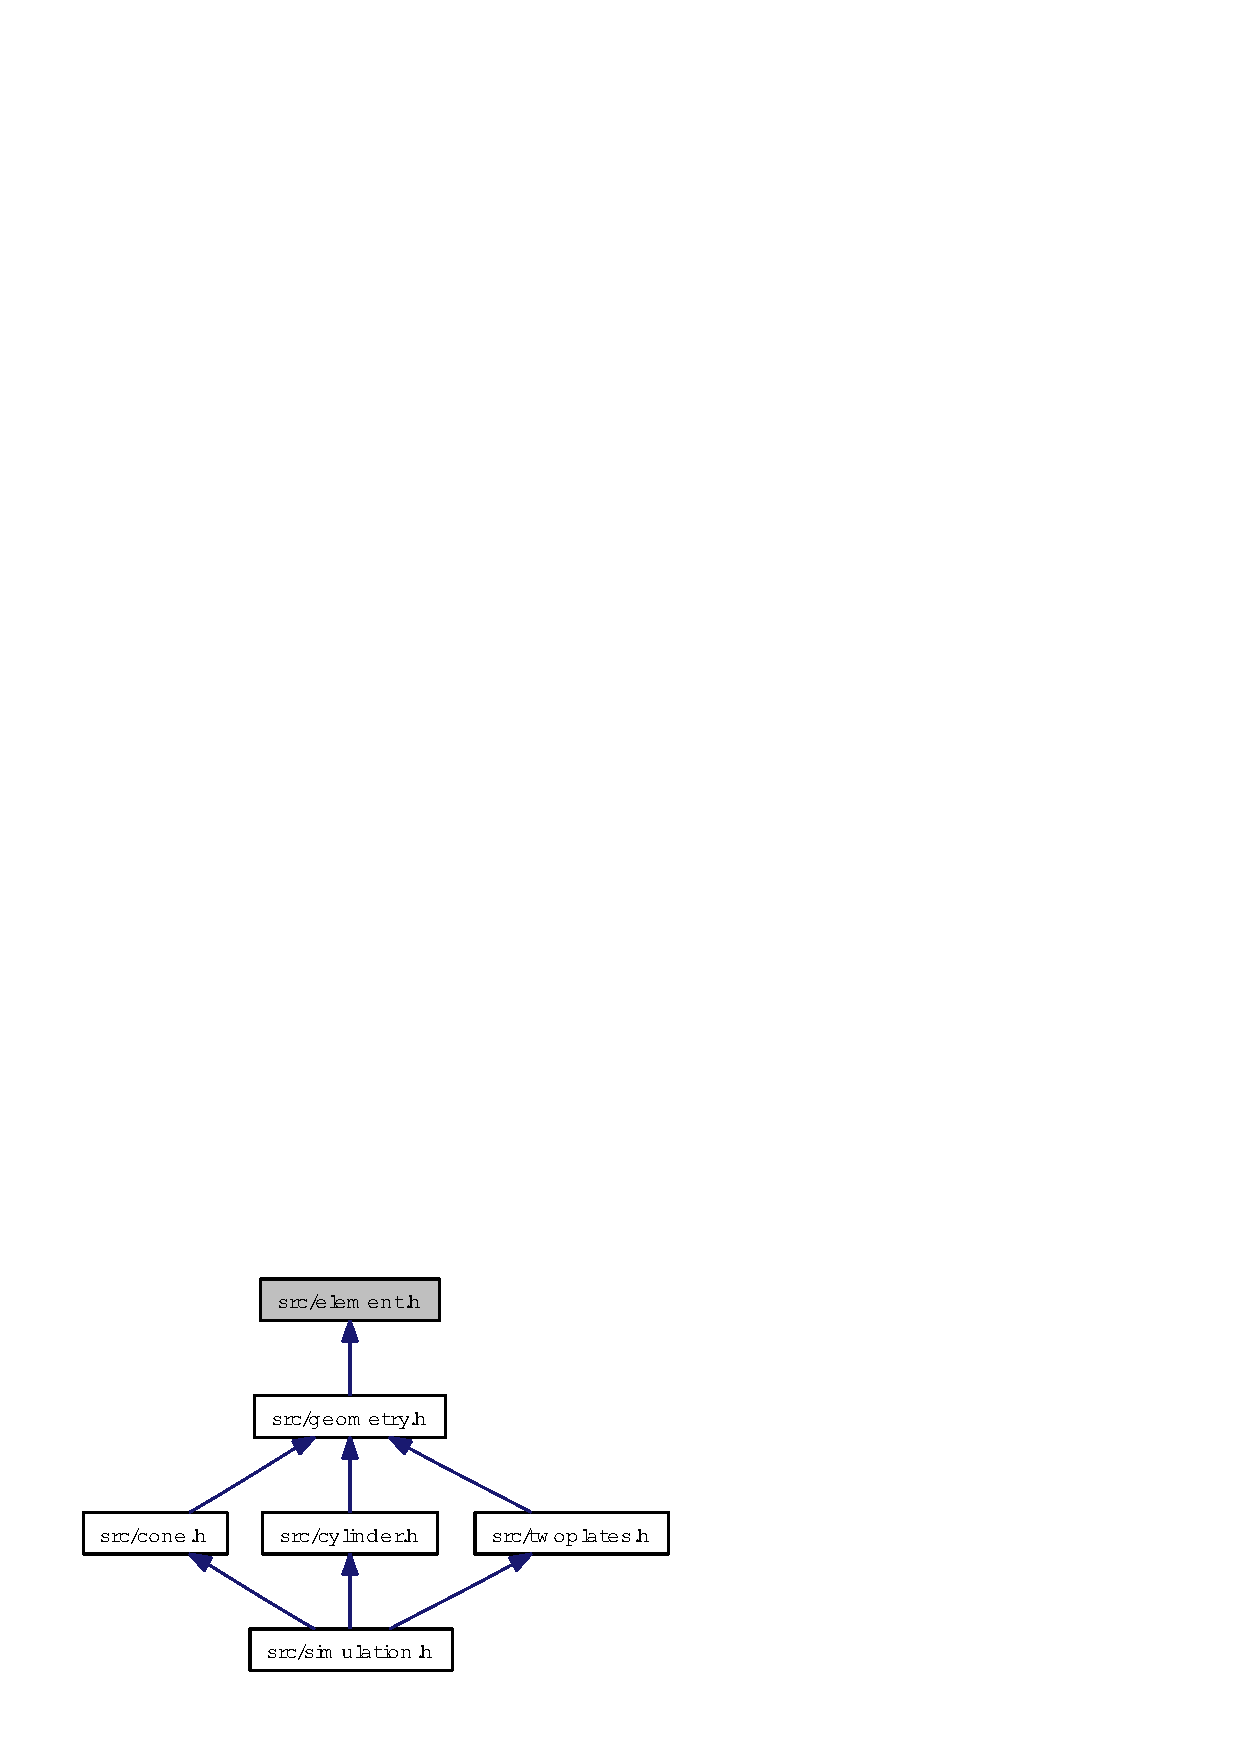
\includegraphics[width=350pt]{element_8h__dep__incl}
\end{center}
\end{figure}
\subsection*{Classes}
\begin{DoxyCompactItemize}
\item 
class \hyperlink{classElement}{Element}
\end{DoxyCompactItemize}


\subsection{Detailed Description}
Facet planar geometry for graphical representation purposes. Uses the \hyperlink{classNode}{Node} class for the defining the vertices. Usually, the dimensions are proportional to the number of sections (longitudinal) and sectors (transversal divisions).

\begin{DoxyAuthor}{Author}
Daniel Iglesias \href{mailto:daniel.iglesias@ciemat.es}{\tt daniel.\-iglesias@ciemat.\-es} 
\end{DoxyAuthor}

\hypertarget{geometry_8h}{\section{src/geometry.h File Reference}
\label{geometry_8h}\index{src/geometry.\-h@{src/geometry.\-h}}
}


Base class for the different geometries.  


{\ttfamily \#include $<$iostream$>$}\\*
{\ttfamily \#include $<$vector$>$}\\*
{\ttfamily \#include $<$map$>$}\\*
{\ttfamily \#include $<$cmath$>$}\\*
{\ttfamily \#include $<$L\-M\-X/lmx.\-h$>$}\\*
{\ttfamily \#include $<$L\-M\-X/lmx\-\_\-nlsolvers.\-h$>$}\\*
{\ttfamily \#include \char`\"{}particle.\-h\char`\"{}}\\*
{\ttfamily \#include \char`\"{}element.\-h\char`\"{}}\\*
{\ttfamily \#include \char`\"{}node.\-h\char`\"{}}\\*
Include dependency graph for geometry.\-h\-:
\nopagebreak
\begin{figure}[H]
\begin{center}
\leavevmode
\includegraphics[width=350pt]{geometry_8h__incl}
\end{center}
\end{figure}
This graph shows which files directly or indirectly include this file\-:\nopagebreak
\begin{figure}[H]
\begin{center}
\leavevmode
\includegraphics[width=350pt]{geometry_8h__dep__incl}
\end{center}
\end{figure}
\subsection*{Classes}
\begin{DoxyCompactItemize}
\item 
class \hyperlink{classGeometry}{Geometry}
\end{DoxyCompactItemize}


\subsection{Detailed Description}
Base class for the different geometries. Abstract class, cannot be instantiated.

\begin{DoxyAuthor}{Author}
Daniel Iglesias \href{mailto:daniel.iglesias@ciemat.es}{\tt daniel.\-iglesias@ciemat.\-es} 
\end{DoxyAuthor}

\hypertarget{node_8h}{
\section{src/node.h File Reference}
\label{node_8h}\index{src/node.h@{src/node.h}}
}
\hyperlink{classNode}{Node} class for graphical representation purposes. 



This graph shows which files directly or indirectly include this file:\nopagebreak
\begin{figure}[H]
\begin{center}
\leavevmode
\includegraphics[width=162pt]{node_8h__dep__incl}
\end{center}
\end{figure}
\subsection*{Classes}
\begin{CompactItemize}
\item 
class \hyperlink{classNode}{Node}
\end{CompactItemize}


\subsection{Detailed Description}
\hyperlink{classNode}{Node} class for graphical representation purposes. 

Simple point definition and manipulation. It has a scalar property for storing the power density.

\begin{Desc}
\item[Author:]Daniel Iglesias $<$\href{mailto:daniel.iglesias@ciemat.es}{\tt daniel.iglesias@ciemat.es}$>$ \end{Desc}

\hypertarget{particle_8h}{\section{src/particle.h File Reference}
\label{particle_8h}\index{src/particle.\-h@{src/particle.\-h}}
}


Represents each of the finite charged particles.  


{\ttfamily \#include $<$iostream$>$}\\*
Include dependency graph for particle.\-h\-:\nopagebreak
\begin{figure}[H]
\begin{center}
\leavevmode
\includegraphics[width=150pt]{particle_8h__incl}
\end{center}
\end{figure}
This graph shows which files directly or indirectly include this file\-:\nopagebreak
\begin{figure}[H]
\begin{center}
\leavevmode
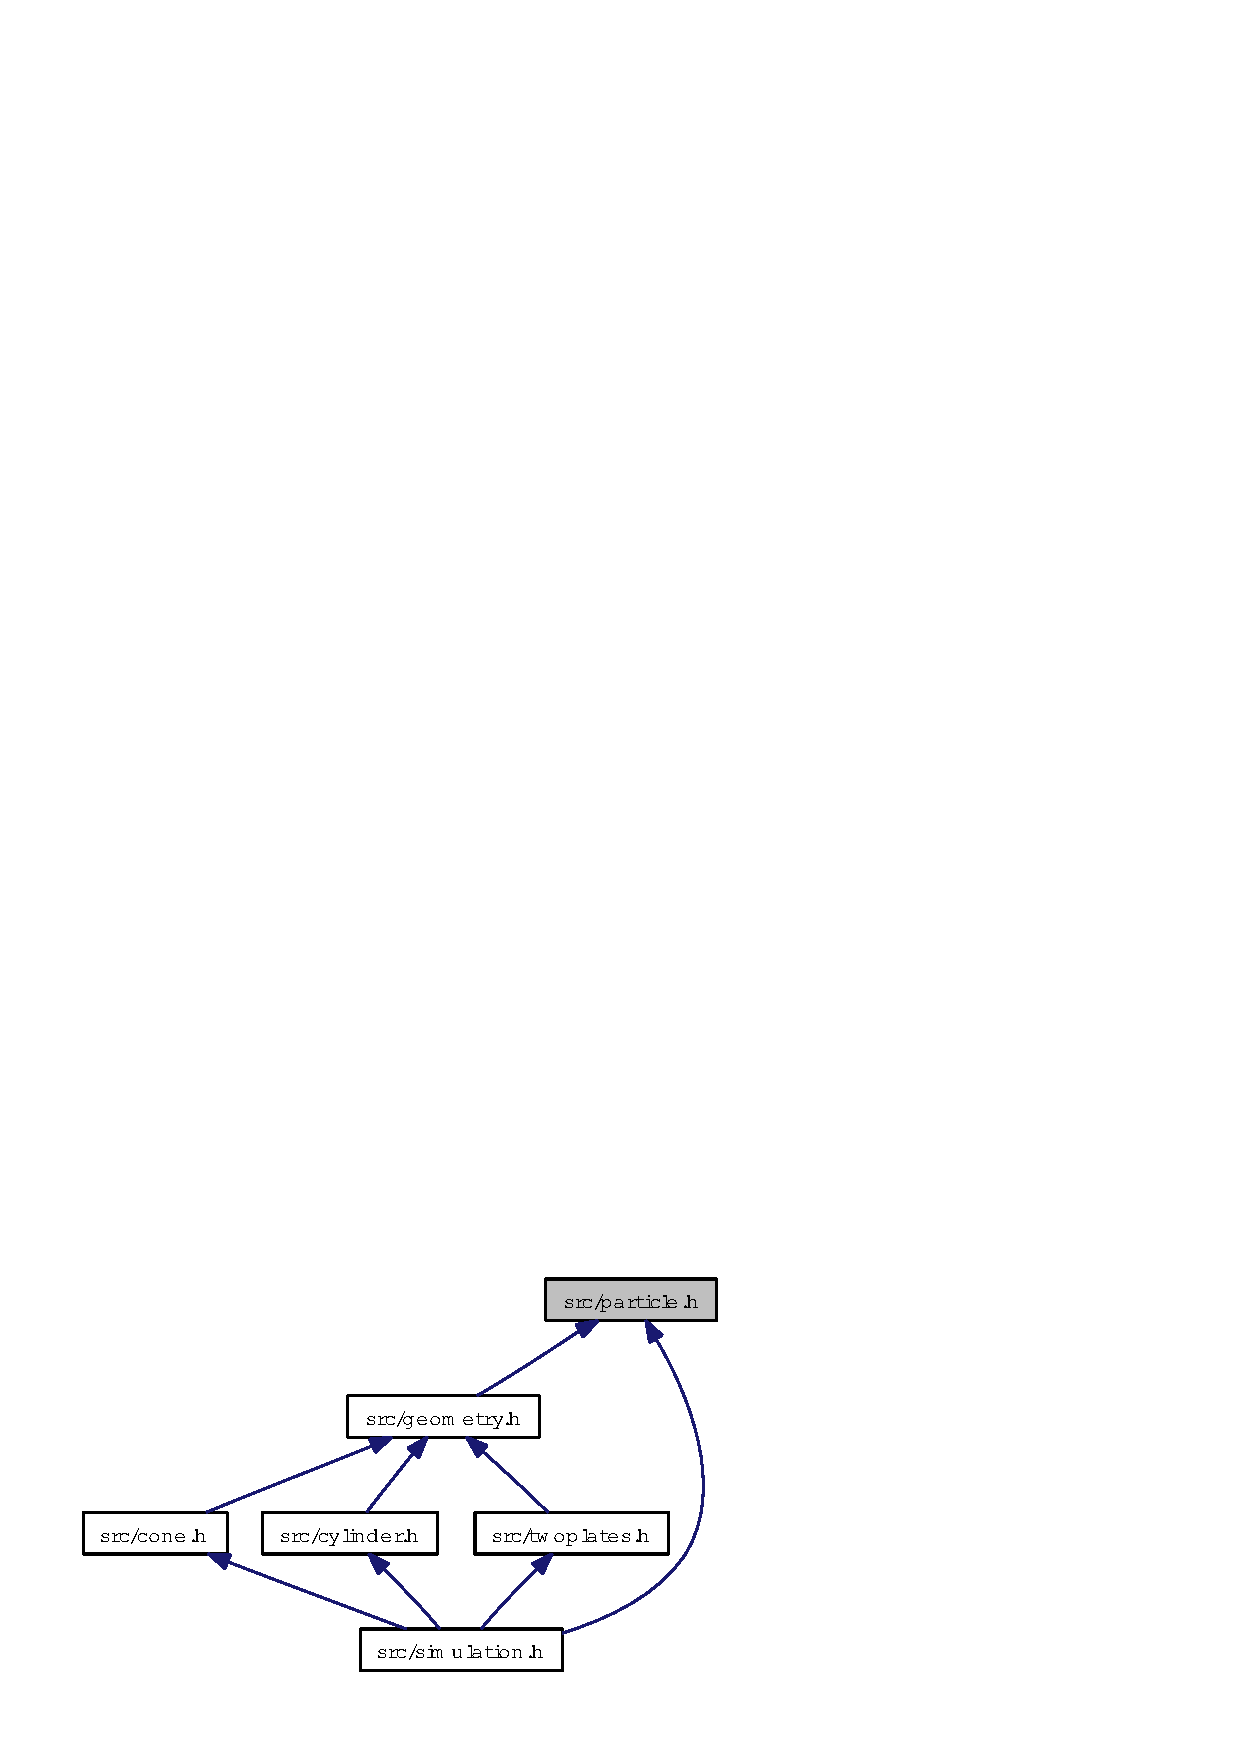
\includegraphics[width=350pt]{particle_8h__dep__incl}
\end{center}
\end{figure}
\subsection*{Classes}
\begin{DoxyCompactItemize}
\item 
class \hyperlink{classParticle}{Particle}
\end{DoxyCompactItemize}


\subsection{Detailed Description}
Represents each of the finite charged particles. Very basic class with stored the x-\/y position in the plane section and the energy of the particle.

\begin{DoxyAuthor}{Author}
Daniel Iglesias \href{mailto:daniel.iglesias@ciemat.es}{\tt daniel.\-iglesias@ciemat.\-es} 
\end{DoxyAuthor}

\hypertarget{simulation_8h}{
\section{src/simulation.h File Reference}
\label{simulation_8h}\index{src/simulation.h@{src/simulation.h}}
}
Procedures for the program workflow. 

{\tt \#include $<$fstream$>$}\par
{\tt \#include $<$vector$>$}\par
{\tt \#include $<$map$>$}\par
{\tt \#include \char`\"{}cone.h\char`\"{}}\par
{\tt \#include \char`\"{}cylinder.h\char`\"{}}\par
{\tt \#include \char`\"{}twoplates.h\char`\"{}}\par
{\tt \#include \char`\"{}particle.h\char`\"{}}\par


Include dependency graph for simulation.h:\nopagebreak
\begin{figure}[H]
\begin{center}
\leavevmode
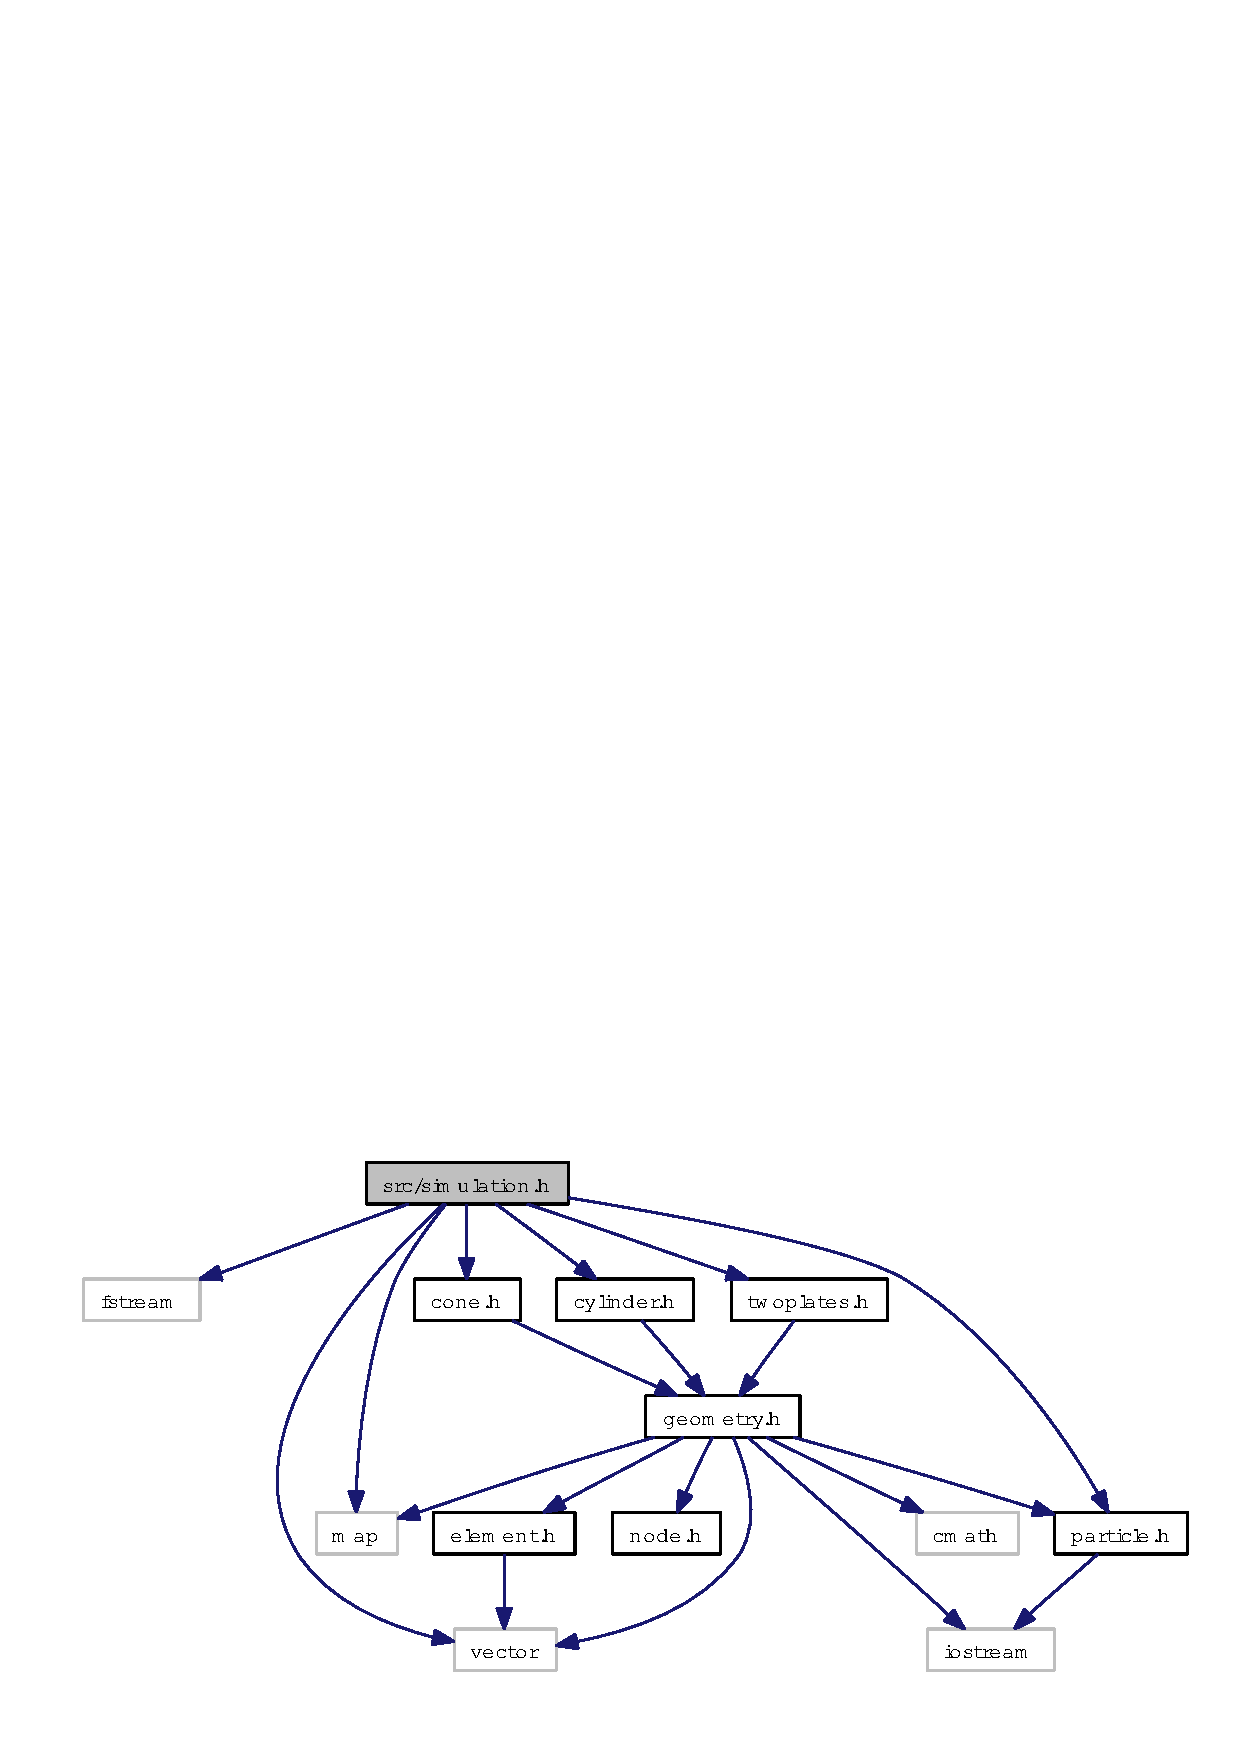
\includegraphics[width=287pt]{simulation_8h__incl}
\end{center}
\end{figure}
\subsection*{Classes}
\begin{CompactItemize}
\item 
class \hyperlink{classSimulation}{Simulation}
\end{CompactItemize}


\subsection{Detailed Description}
Procedures for the program workflow. 

Reads files, creates all of the objects, lauches the computation and creates the output.

\begin{Desc}
\item[Author:]Daniel Iglesias $<$\href{mailto:daniel.iglesias@ciemat.es}{\tt daniel.iglesias@ciemat.es}$>$ \end{Desc}

\hypertarget{twoplates_8h}{\section{src/twoplates.h File Reference}
\label{twoplates_8h}\index{src/twoplates.\-h@{src/twoplates.\-h}}
}


Two symmetrical plates geometry.  


{\ttfamily \#include $<$geometry.\-h$>$}\\*
Include dependency graph for twoplates.\-h\-:
\nopagebreak
\begin{figure}[H]
\begin{center}
\leavevmode
\includegraphics[width=350pt]{twoplates_8h__incl}
\end{center}
\end{figure}
This graph shows which files directly or indirectly include this file\-:\nopagebreak
\begin{figure}[H]
\begin{center}
\leavevmode
\includegraphics[width=326pt]{twoplates_8h__dep__incl}
\end{center}
\end{figure}
\subsection*{Classes}
\begin{DoxyCompactItemize}
\item 
class \hyperlink{classTwoPlates}{Two\-Plates}
\end{DoxyCompactItemize}


\subsection{Detailed Description}
Two symmetrical plates geometry. \hyperlink{classGeometry}{Geometry} with origin in s=0 defined by s-\/length and initial plate separation (constant slope).

\begin{DoxyAuthor}{Author}
Daniel Iglesias \href{mailto:daniel.iglesias@ciemat.es}{\tt daniel.\-iglesias@ciemat.\-es} 
\end{DoxyAuthor}

\printindex
\end{document}
